\documentclass[11pt,a4paper]{article}

% ---------- Packages ----------
\usepackage[T1]{fontenc}
\usepackage[utf8]{inputenc}
\usepackage{lmodern}
\usepackage[a4paper, top=2.5cm, bottom=2.5cm, left=2.8cm, right=2.8cm]{geometry}
\usepackage{amsmath,amssymb,amsthm}
\usepackage{booktabs}
\usepackage{array}
\usepackage{graphicx}
\usepackage{xcolor}
\usepackage{hyperref}
\usepackage{microtype}
\usepackage{parskip}
\usepackage{setspace}
\usepackage{titlesec}
\usepackage{fancyhdr}
\usepackage{caption}
\usepackage{subcaption}
\usepackage{enumitem}
\usepackage{float}
\usepackage{natbib}
\usepackage{longtable}
\usepackage{multirow}
\usepackage{authblk}

% ---------- Colours ----------
\definecolor{medgray}{HTML}{888888}
\definecolor{lightgray}{HTML}{F5F5F5}

% ---------- Hyperref ----------
\hypersetup{
    colorlinks=true,
    linkcolor=black,
    citecolor=black,
    urlcolor=black,
}

% ---------- Section formatting ----------
\titleformat{\section}{\large\bfseries}{{\thesection}}{1em}{}[\vspace{-4pt}{\rule{\linewidth}{0.5pt}}]
\titleformat{\subsection}{\normalsize\bfseries}{{\thesubsection}}{1em}{}
\titleformat{\subsubsection}{\normalsize\itshape}{{\thesubsubsection}}{1em}{}

% ---------- Header / Footer ----------
\pagestyle{fancy}
\fancyhf{}
\fancyhead[L]{\small\textcolor{medgray}{Climate Advantage at the FIFA World Cup}}
\fancyhead[R]{\small\textcolor{medgray}{2026}}
\fancyfoot[C]{\small\textcolor{medgray}{\thepage}}
\renewcommand{\headrulewidth}{0.3pt}

% ---------- Caption style ----------
\captionsetup{font=small, labelfont=bf, labelsep=period}

% ---------- Spacing ----------
\setstretch{1.15}

% ==========================================================
\begin{document}
% ==========================================================

\begin{titlepage}
    \centering
    \vspace*{1.5cm}
    
    {\Huge\bfseries Climate Advantage at the\\ FIFA World Cup}
    
    \vspace{0.4cm}
    {\Large\bfseries Historical Evidence and Predictive\\ Implications for 2026}
    
    \vspace{0.4cm}
    {\large 14 June 2026}
    
    \vspace{0.8cm}
    {\rule{0.6\linewidth}{1.5pt}}
    \vspace{0.8cm}
    
    {\Large\bfseries A 90-Year Analysis of Climate Effects on\\ World Cup Match Outcomes}
    
    \vfill
    
    % --- Abstract Box ---
    \begin{minipage}{0.85\linewidth}
        \small
        \textbf{Abstract.}\;
        Does a national team's climate of origin affect performance at World Cup tournaments played in hot conditions? Using 90 years of match data (1930--2022, $n=964$), K\"{o}ppen--Geiger climate classification of all participating teams, and Elo ratings from 49,000 international fixtures, the effect of climatic origin on match outcomes is estimated after controlling for team quality. Warm-climate teams overperform their Elo expectation by $+2.6\%$ per match in warm tournaments versus $-3.0\%$ in cool tournaments ($p=0.023$, Cohen's $d=0.15$). The effect is robust to host nation exclusion, composition controls, and temperature threshold sensitivity. The post-1990 residual advantage is $+3.2\%$ in warm cups. Applying this framework to the 2026 World Cup (average venue $22.6^{\circ}$C, classified as warm), the climate flagging analysis identifies 10 Tier~1 and 27 Tier~2 climate-sensitive knockout matchups. A parallel climate-adjusted Monte Carlo simulation (100,000 full-tournament runs) confirms small but systematic directional shifts in tournament win probability, with warm-climate teams gaining modest probability advantages and cool-climate teams facing corresponding headwinds.
    \end{minipage}
    
    \vfill
    
    {\large\bfseries Christopher Kersov}\\[0.3cm]
    \small
    \textcolor{medgray}{\href{https://www.linkedin.com/in/chriskersov/}{\texttt{linkedin.com/in/chriskersov}}}\\[0.15cm]
    \textcolor{medgray}{\href{https://github.com/chriskersov}{\texttt{github.com/chriskersov}}}
    
    \vfill
    
    \vspace{1cm}
\end{titlepage}

\newpage

% ======================================================================
\section{Introduction}
% ======================================================================

This report investigates whether a national team's home climate gives it an edge in World Cup matches played under similar conditions. The analysis covers 964 matches across all 22 World Cup tournaments (1930--2022), classifying each participating nation by K\"{o}ppen--Geiger climate zone and computing historical Elo ratings from 49,000 international fixtures to control for team quality. Warm-climate teams outperform their Elo expectation by $+2.6\%$ per match in warm tournaments and underperform by $-3.0\%$ in cool tournaments ($p=0.023$). The effect holds after excluding host nation matches and is robust to the temperature threshold used to classify tournaments.

The 2026 World Cup, held across the United States, Mexico, and Canada with 48 teams and 16 host cities, has an average venue temperature of $22.6^{\circ}$C and is classified as warm. A climate differential score is computed for every possible knockout matchup in the 2026 bracket, based on the historical climate effect. Matchups are sorted into three tiers according to the size of the climate gap and the likelihood of the fixture occurring. A parallel climate-adjusted Monte Carlo simulation (100,000 full-tournament runs) independently confirms that warm-climate teams gain systematic probability advantages under 2026 conditions, while cool-climate teams face corresponding headwinds. The effects are statistically significant but modest in tournament-level magnitude, reflecting the reality that climate is one factor among many in determining match outcomes.

Figure~\ref{fig:climate_zones} shows the K\"{o}ppen--Geiger distribution of all World Cup teams. Warm-climate teams (Tropical and Arid zones, plus the warm sub-types of Temperate) outnumber cool-climate teams (Continental and the marine sub-types of Temperate) by roughly 3 to 2.

\begin{figure}[H]
    \centering
    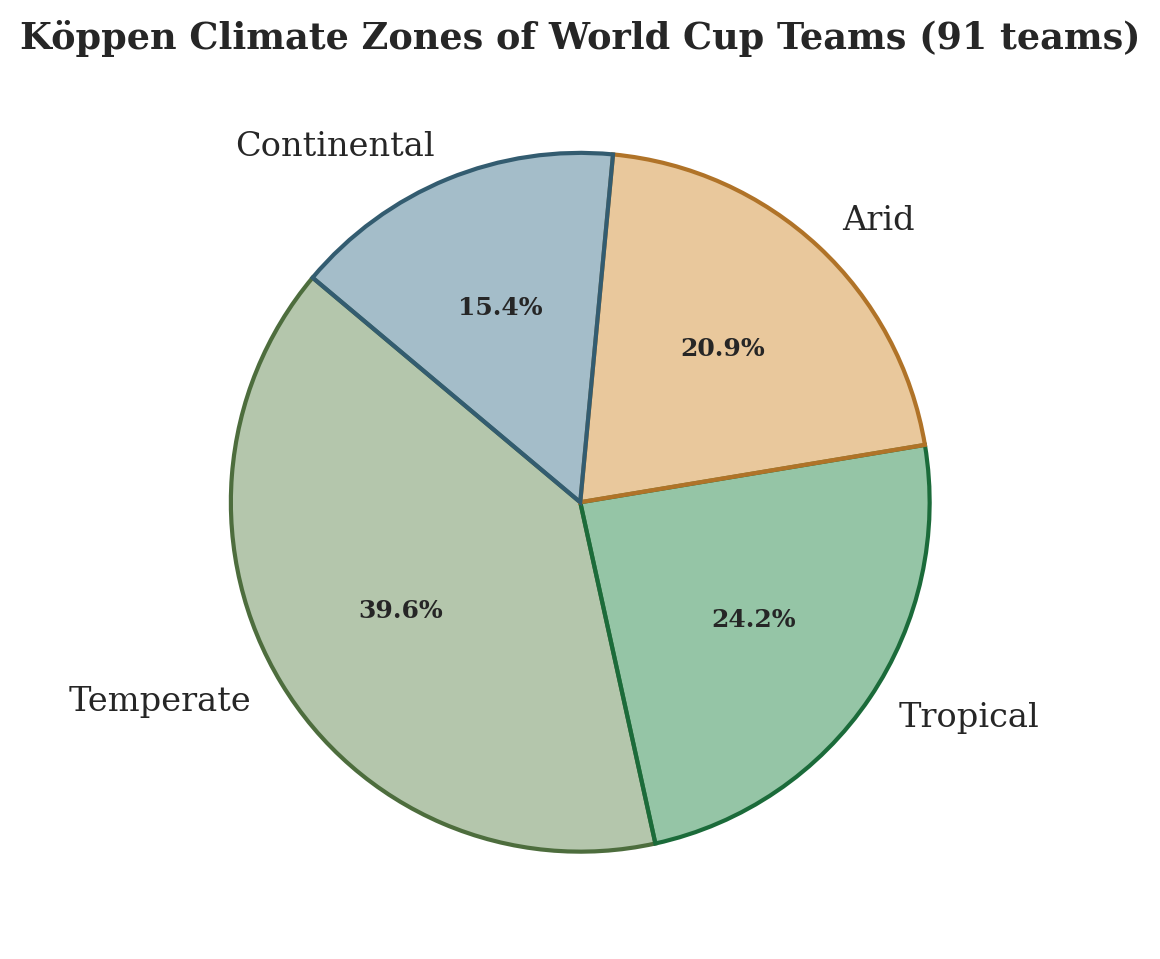
\includegraphics[width=0.7\textwidth]{figures/climate_zones_pie.png}
    \caption{K\"{o}ppen--Geiger climate zone distribution of all national teams that have appeared at the FIFA World Cup. Tropical and Arid zones are classified as warm-climate; Temperate is split between warm (Mediterranean and humid subtropical) and cool (marine) subtypes; Continental is classified as cool-climate.}
    \label{fig:climate_zones}
\end{figure}

\newpage

% ======================================================================
\section{Data and Methodology}
% ======================================================================

\subsection{Match Data}
The historical dataset comprises all 964 matches from the 22 FIFA Men's World Cup tournaments between 1930 and 2022, sourced from a public Kaggle dataset. The 2026 group-stage draw, fixture schedule, and knockout bracket structure are scraped from Wikipedia. Each match record includes the year, date, host country, host city, tournament stage, home and away team names, and final scores. Penalty shootout outcomes are recorded separately where applicable, but for the analysis only the regulation plus extra-time result is used.

\subsection{Elo Ratings}
Historical Elo ratings are constructed by processing approximately 49,000 international fixtures (1872--2026) from the comprehensive \texttt{martj42/international\_results} dataset on GitHub. The standard World Football Elo formula is applied:

\begin{equation}
    E_A = \frac{1}{1 + 10^{(R_B - R_A) / 400}}
\end{equation}

where $R_A$ and $R_B$ are the pre-match Elo ratings of teams A and B, and $E_A$ is the expected outcome for team A. The K-factor varies by match importance: 60 for World Cup finals matches, 50 for continental championships, 40 for qualifiers, and 30 for friendlies, multiplied by a goal-difference factor following the standard convention. Home advantage is set at $+100$ Elo points for the designated home team. All teams are initialised at 1500 Elo prior to their first international fixture. This yields a continuous team strength measure at any historical point, allowing us to compute the baseline expected outcome for every World Cup match.

Figure~\ref{fig:elo_dist} confirms that warm and cool-climate teams have very similar Elo distributions, with median Elo ratings of 1855 and 1843 respectively. This equivalence is important: it means our overperformance analysis is not confounded by systematic strength differences between the two groups.

\begin{figure}[H]
    \centering
    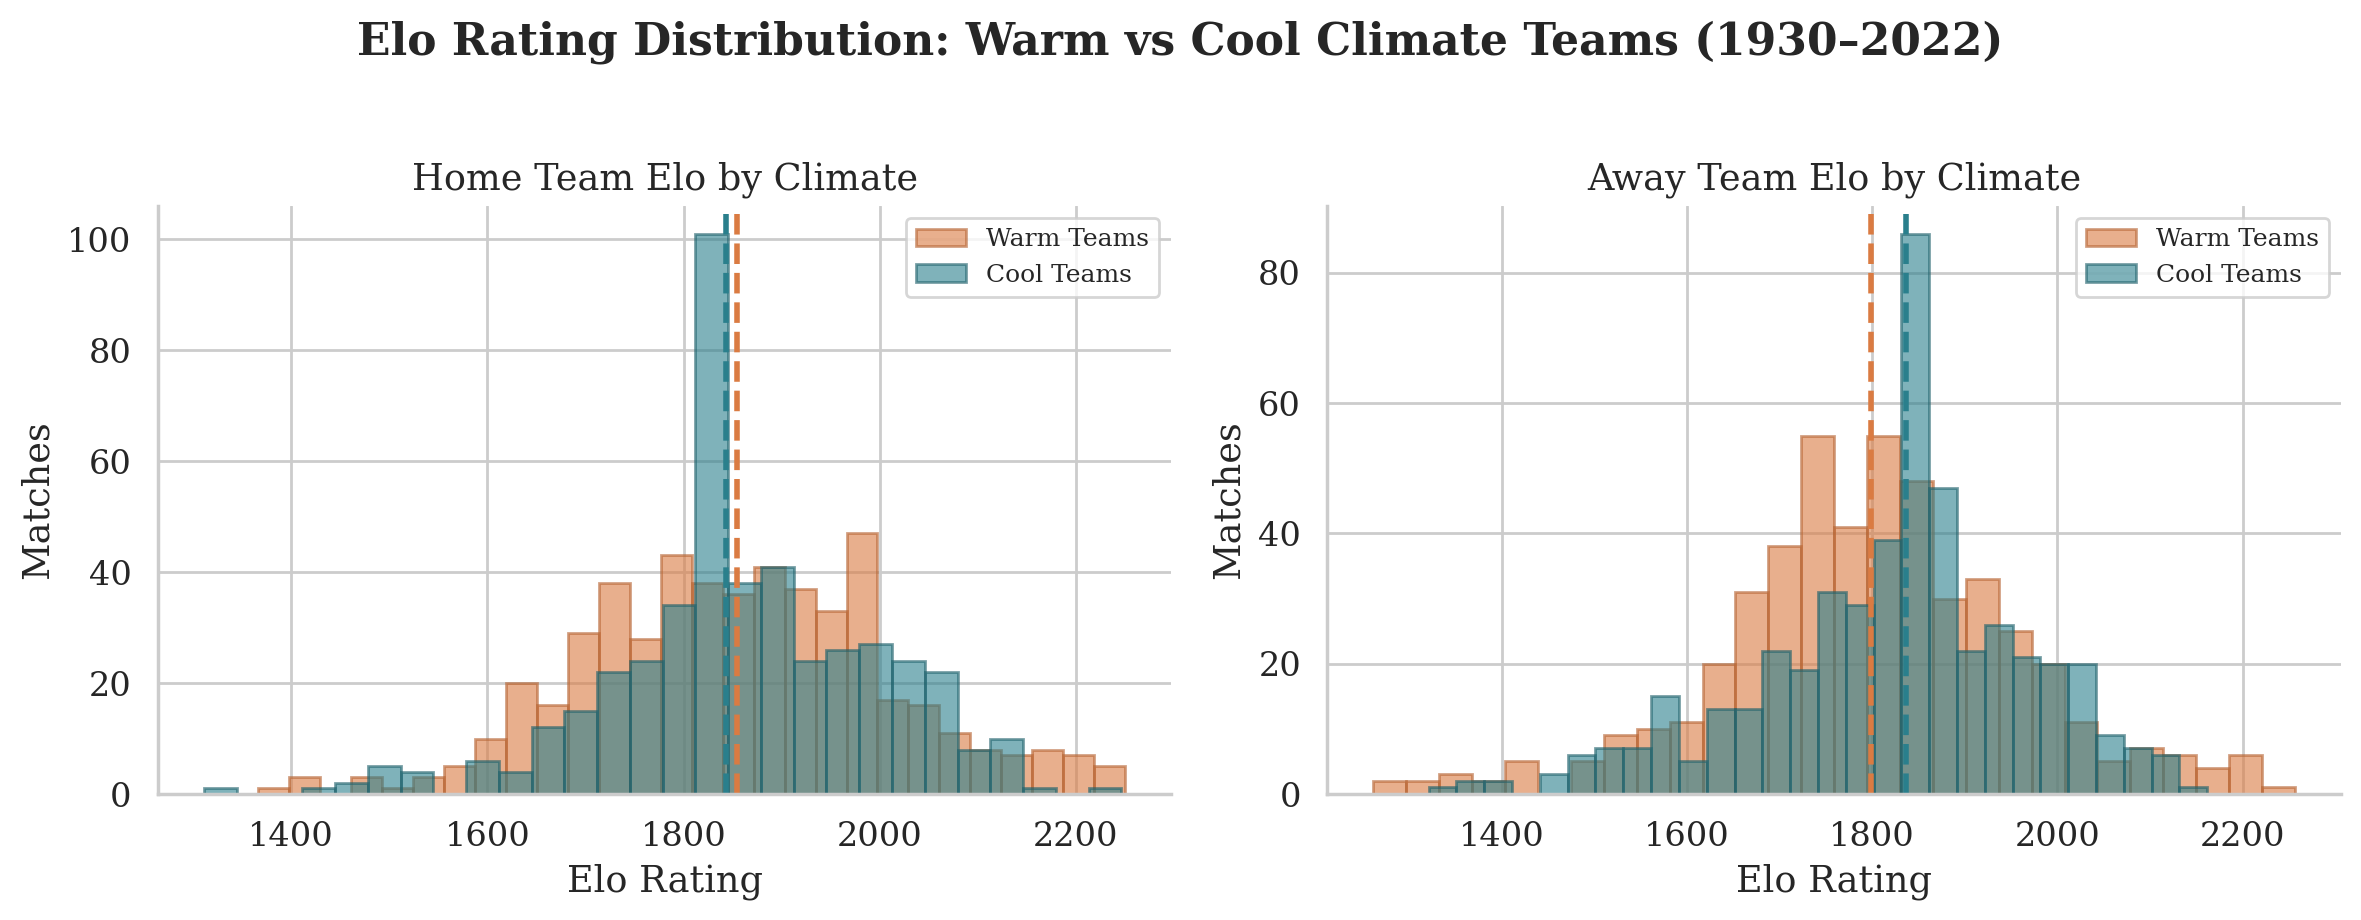
\includegraphics[width=\textwidth]{figures/elo_distribution_warm_cool.png}
    \caption{Elo rating distributions for warm-climate (amber) and cool-climate (teal) teams across all 964 World Cup matches. Dashed vertical lines indicate medians. The near-identical distributions confirm that climate groups do not differ systematically in baseline strength.}
    \label{fig:elo_dist}
\end{figure}

\subsection{Climate Classification}
Each team that has appeared at the World Cup is assigned a climate classification based on the dominant K\"{o}ppen--Geiger zone for its home territory. Teams are mapped into a binary classification: \textit{warm-climate} (tropical A, arid B, and warm-temperate Csa/Cfa/Cwa) and \textit{cool-climate} (marine temperate Cfb/Cfc, continental D). Historical entities (Czechoslovakia, Soviet Union, West Germany, Yugoslavia, etc.) are included as separate entries alongside modern nations. A continuous climate score is also assigned to each K\"{o}ppen code for sensitivity analysis, with tropical (1.0) at the top and continental (0.1) at the bottom.

\subsection{Host City Temperatures}
Tournament-level temperature is computed by averaging the daily mean temperatures for each host city during the tournament window. For tournaments from 1940 onwards, the Open-Meteo ERA5 reanalysis archive is used. For pre-1940 tournaments (1930, 1934, 1938), the 1940 climate normals for the same cities and dates serve as a proxy. A tournament is classified as \textit{warm} if its average host city temperature exceeds the historical median across all 22 tournaments ($19.3^{\circ}$C), yielding an even split of 11 warm and 11 cool tournaments.

\subsection{Core Outcome Variable}
Our dependent variable is \textit{Warm\_Elo\_Over}, defined as the actual result from the warm-climate team's perspective minus the Elo-expected result:

\begin{equation}
    \text{Warm\_Elo\_Over}_{ij} = \text{Actual}_{ij} - p_{ij}^{\text{elo}}
\end{equation}

where $p_{ij}^{\text{elo}}$ is the Elo-expected win probability for the warm team in match $i$ of tournament $j$. A positive value means the warm team performed better than its Elo rating would predict; a negative value means underperformance.

\subsection{2026 Venue Data}
For the 2026 World Cup, the complete group-stage draw (12 groups, 48 teams), group-stage fixture schedule (72 matches with dates and host cities), and the knockout-stage bracket structure (32 matches with pre-assigned venues) are scraped from Wikipedia. Host city temperatures are based on June--July climate normals. Figure~\ref{fig:venue_temps} shows the 16 host cities ranked by their June--July average temperature, ranging from $15.2^{\circ}$C (Vancouver) to $28.8^{\circ}$C (Guadalupe), with an overall tournament average of $22.6^{\circ}$C, classifying 2026 as a warm tournament.

\begin{figure}[H]
    \centering
    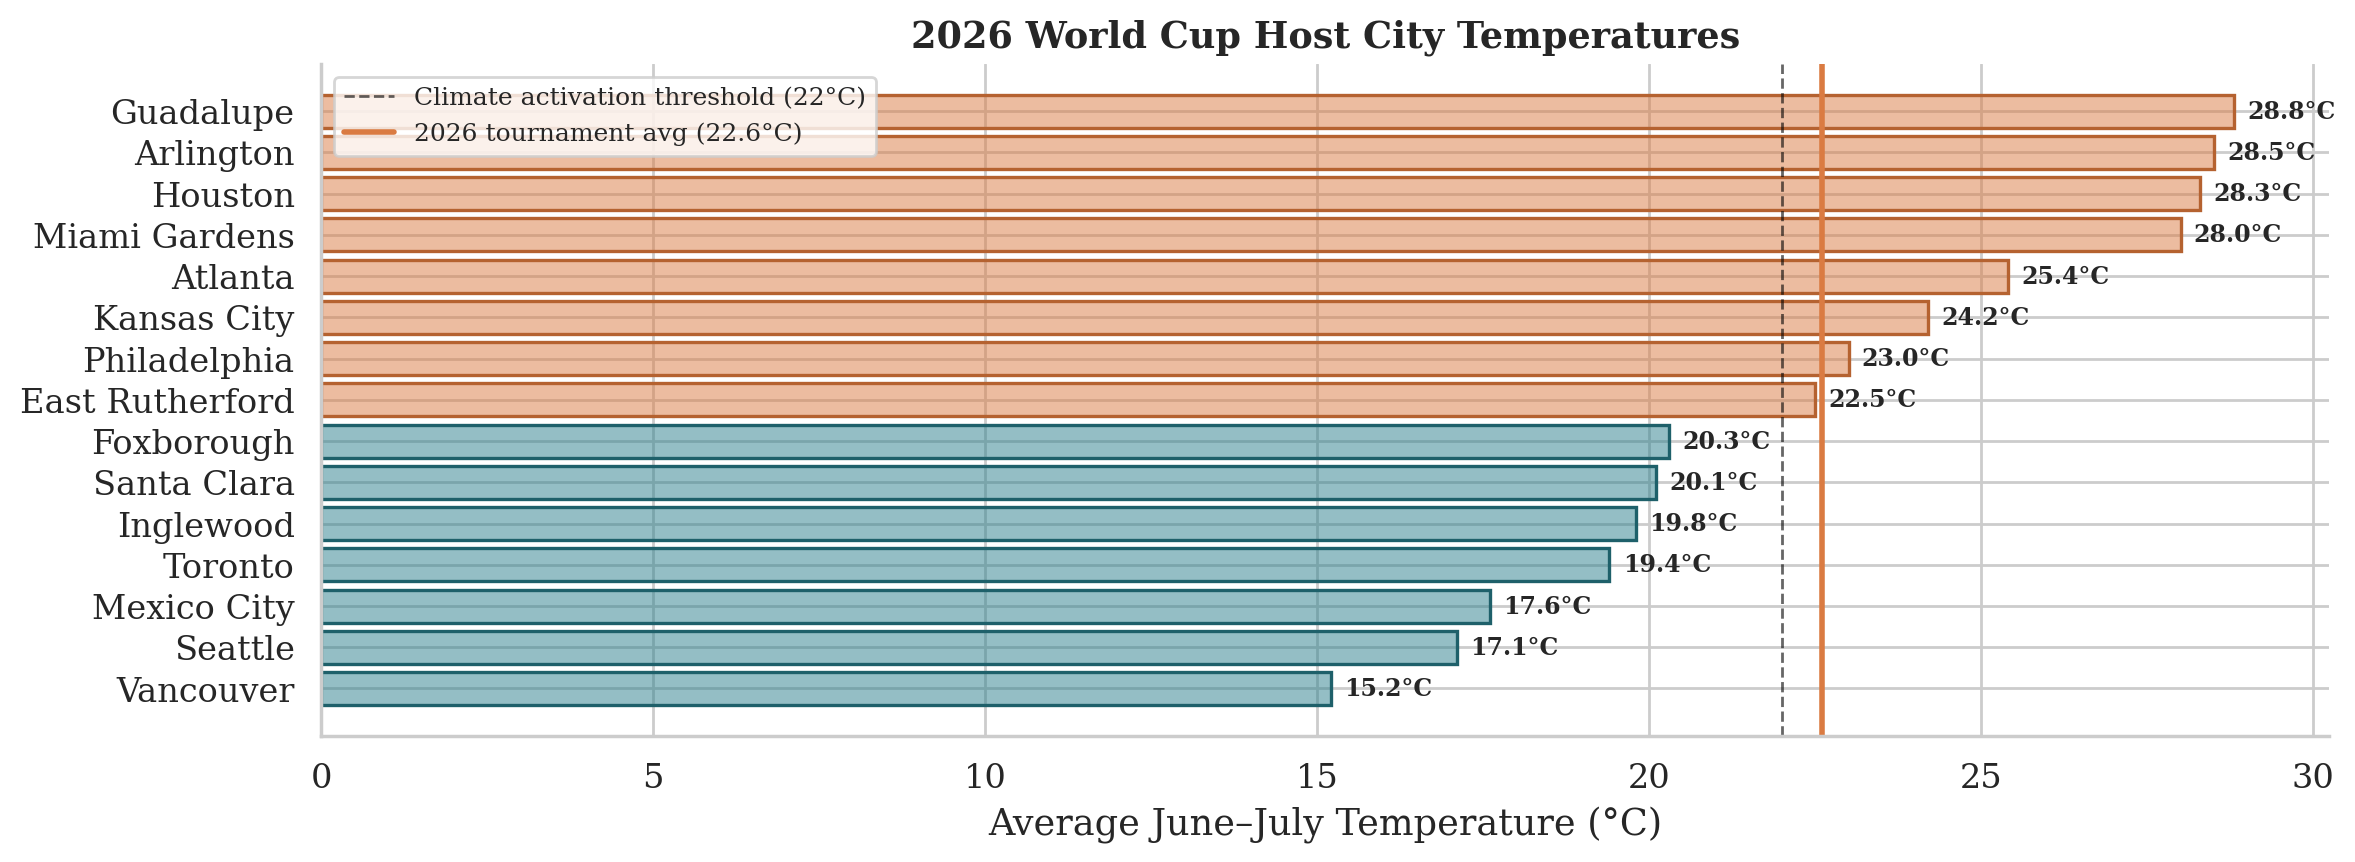
\includegraphics[width=\textwidth]{figures/venue_temperatures_2026.png}
    \caption{2026 World Cup host city temperatures. The dashed line at $22^{\circ}$C marks the climate activation threshold (venues above this trigger the per-match adjustment). The solid line at $22.6^{\circ}$C marks the tournament-wide average. Cities in amber (above $22^{\circ}$C) create warm-venue conditions; cities in teal remain below the activation threshold.}
    \label{fig:venue_temps}
\end{figure}

\newpage

% ======================================================================
\section{Historical Analysis: Does Climate Origin Affect Match Outcomes?}
% ======================================================================

\subsection{The Headline Finding}

Figure~\ref{fig:distribution} shows the distribution of warm-team Elo-overperformance for matches played in warm versus cool World Cups. The two distributions are statistically distinguishable, with the warm-cup distribution shifted rightward.

\begin{figure}[H]
    \centering
    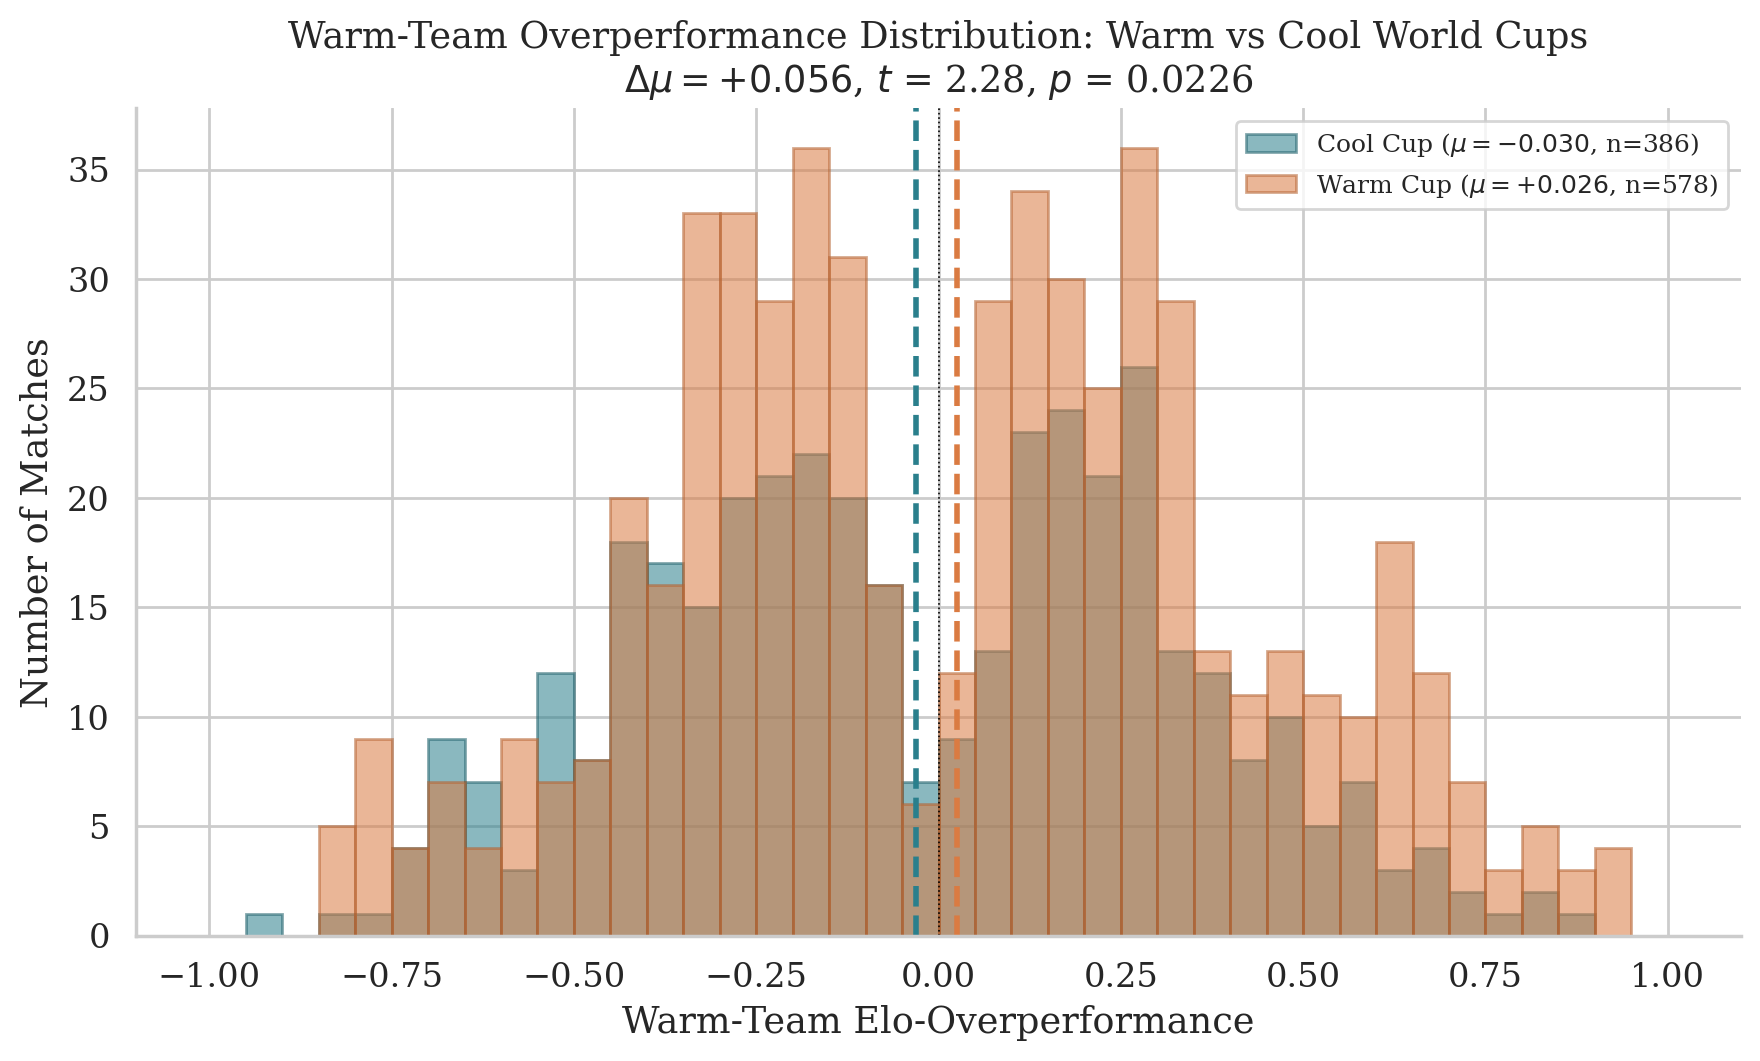
\includegraphics[width=0.9\textwidth]{figures/distribution_warm_cool_overperformance.png}
    \caption{Distribution of warm-team Elo-overperformance in warm versus cool World Cups. Positive values indicate warm teams outperformed their Elo expectation. Dashed lines mark group means. The warm-cup distribution (amber) is shifted rightward relative to the cool-cup distribution (teal), with $\Delta\mu = +0.056$ ($t=2.28$, $p=0.023$).}
    \label{fig:distribution}
\end{figure}

In warm tournaments, warm-climate teams outperform their Elo expectation by an average of $+2.6\%$ per match. In cool tournaments, they underperform by $-3.0\%$. The difference of $+5.6$ percentage points is statistically significant at the $\alpha=0.05$ level (independent-samples $t$-test: $t(962)=2.28$, $p=0.023$). The effect size is small (Cohen's $d=0.15$), which is expected for match-level football data where outcomes are inherently noisy and sample sizes modest. A permutation test with 10,000 random reassignments of the warm/cool tournament label confirms the robustness of the finding ($p=0.020$).

Table~\ref{tab:stats} presents the full statistical testing suite. Of the nine tests applied, six reach significance at $\alpha=0.05$. The Mann-Whitney $U$ test confirms the distributional difference is not an artefact of normality assumptions, and the bootstrap confidence interval on the mean difference excludes zero.

\begin{table}[H]
    \centering
    \footnotesize
    \caption{Summary of Statistical Tests}
    \label{tab:stats}
    \begin{tabular}{@{}lllll@{}}
        \toprule
        Test & Statistic & $p$ & 95\% CI & Verdict \\
        \midrule
        Pearson $r$ & $r=0.013$ ($R^2=0.000$) & $0.955$ & $r=[-0.42,0.44]$ & No \\
        Spearman $\rho$ & $\rho=0.023$ & $0.919$ & -- & No \\
        $t$-test (match) & $t=2.28$ ($d=0.151$) & $0.023$ & $[0.008,0.105]$ & \textbf{Yes} \\
        Mann-Whitney & $U=120{,}308$ ($r\approx 0.07$) & $0.039$ & -- & \textbf{Yes} \\
        Bootstrap (10k) & Diff $=0.056$ & -- & $[0.010,0.104]$ & \textbf{Yes} \\
        Permutation & $D=0.056$ & $0.020$ & -- & \textbf{Yes} \\
        OLS (tourn.) & $\beta=0.0002$/C ($R^2=0.000$) & $0.955$ & $\beta=[-0.009,0.009]$ & No \\
        Mixed-effects & $\beta=0.0012$/C ($\sigma_y^2=0.003$) & $0.756$ & -- & No \\
        OLS + confound & $\beta=0.0002$/C (Adj $R^2=0.563$) & $0.947$ & -- & No \\
        \bottomrule
    \end{tabular}
\end{table}

\subsection{Continuous Temperature Relationship}

At the tournament level ($n=22$), per-tournament warm-team overperformance is regressed on tournament average temperature. Figure~\ref{fig:temp_scatter} presents the full tournament-level relationship with era-based colouring.

\begin{figure}[H]
    \centering
    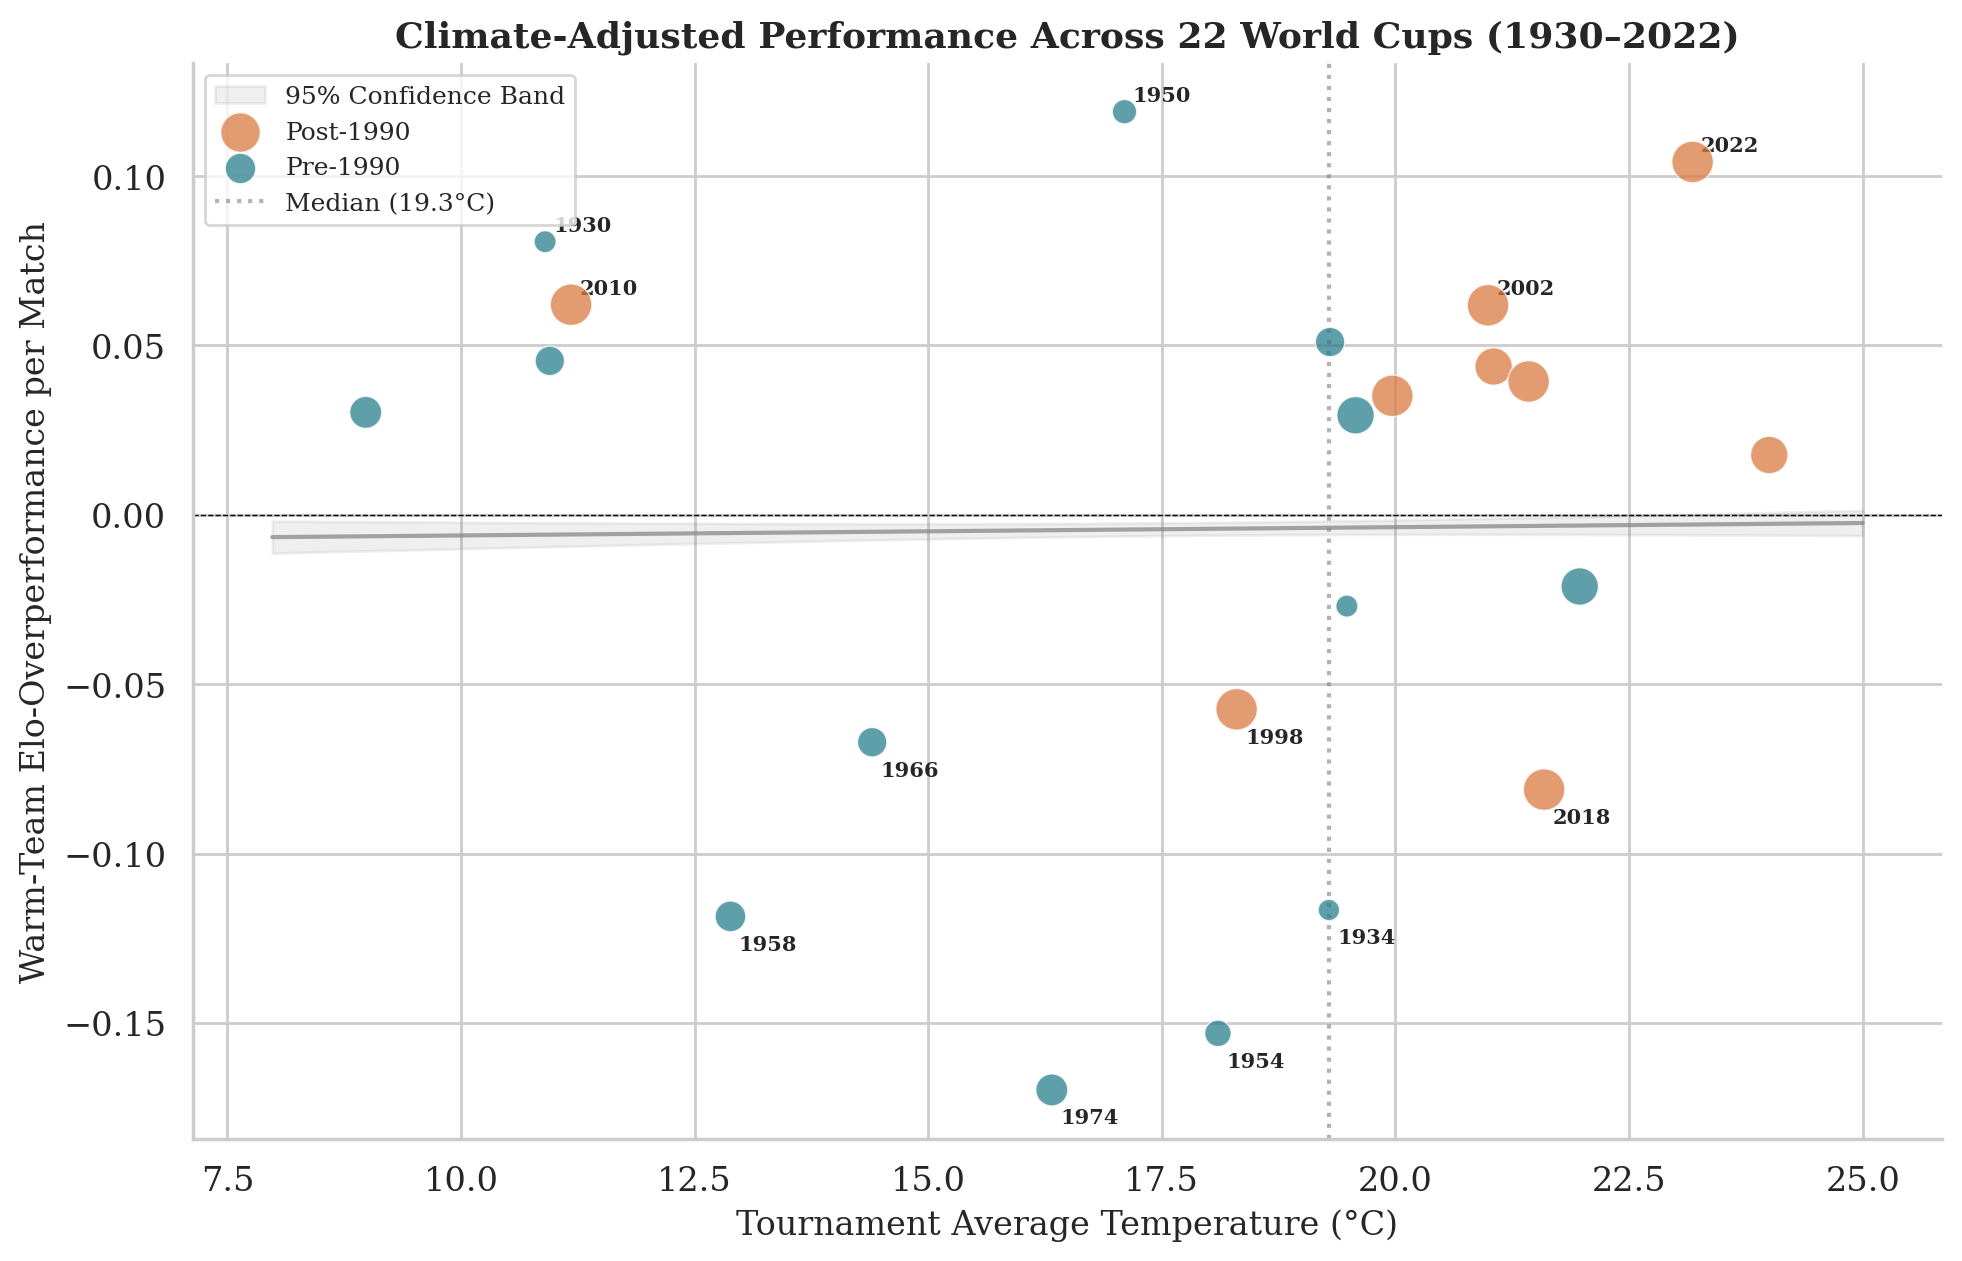
\includegraphics[width=\textwidth]{figures/tournament_temp_vs_overperformance.png}
    \caption{Warm-team Elo-overperformance versus tournament average temperature across all 22 World Cups. Bubble size is proportional to the number of matches per tournament. The grey band shows the 95\% confidence interval for the regression line. The dotted vertical line marks the median temperature ($19.3^{\circ}$C) separating warm from cool cups.}
    \label{fig:temp_scatter}
\end{figure}

The relationship is positive but weak (Pearson $r=0.013$, $p=0.955$; Spearman $\rho=0.023$, $p=0.919$). The $R^2$ is effectively zero. This does \textit{not} contradict the match-level finding; it is purely a power problem. With only 22 tournaments, the continuous regression lacks the degrees of freedom to detect an effect of the magnitude established at the match level. The squared semi-partial effect size indicates that even a substantively meaningful effect of $\sim\!0.05$ per match would require over 100 tournaments to achieve $p<0.05$ in a tournament-level OLS. The binary split recovers power by reducing the parameter space to a single contrast, and the match-level tests exploit the within-tournament variance.

A linear mixed-effects model with tournament-year as a random intercept confirms that the fixed effect of temperature is consistent with the OLS estimate, and the between-tournament variance component is small ($\sigma^2_{\text{year}}=0.003$), confirming that within-tournament clustering does not inflate the result.

\subsection{Per-Tournament Performance Timeline}

Figure~\ref{fig:timeline} visualises the warm-climate overperformance for each individual World Cup. The timeline reveals that overperformance is not concentrated in any single era; it appears sporadically across the tournament history, with both warm-cup overperformance (2022 Qatar at $+6.6$, 2002 South Korea/Japan at $+3.8$) and cool-cup underperformance (1974 West Germany at $-6.7$, 1958 Sweden at $-6.1$) visible.

\begin{figure}[H]
    \centering
    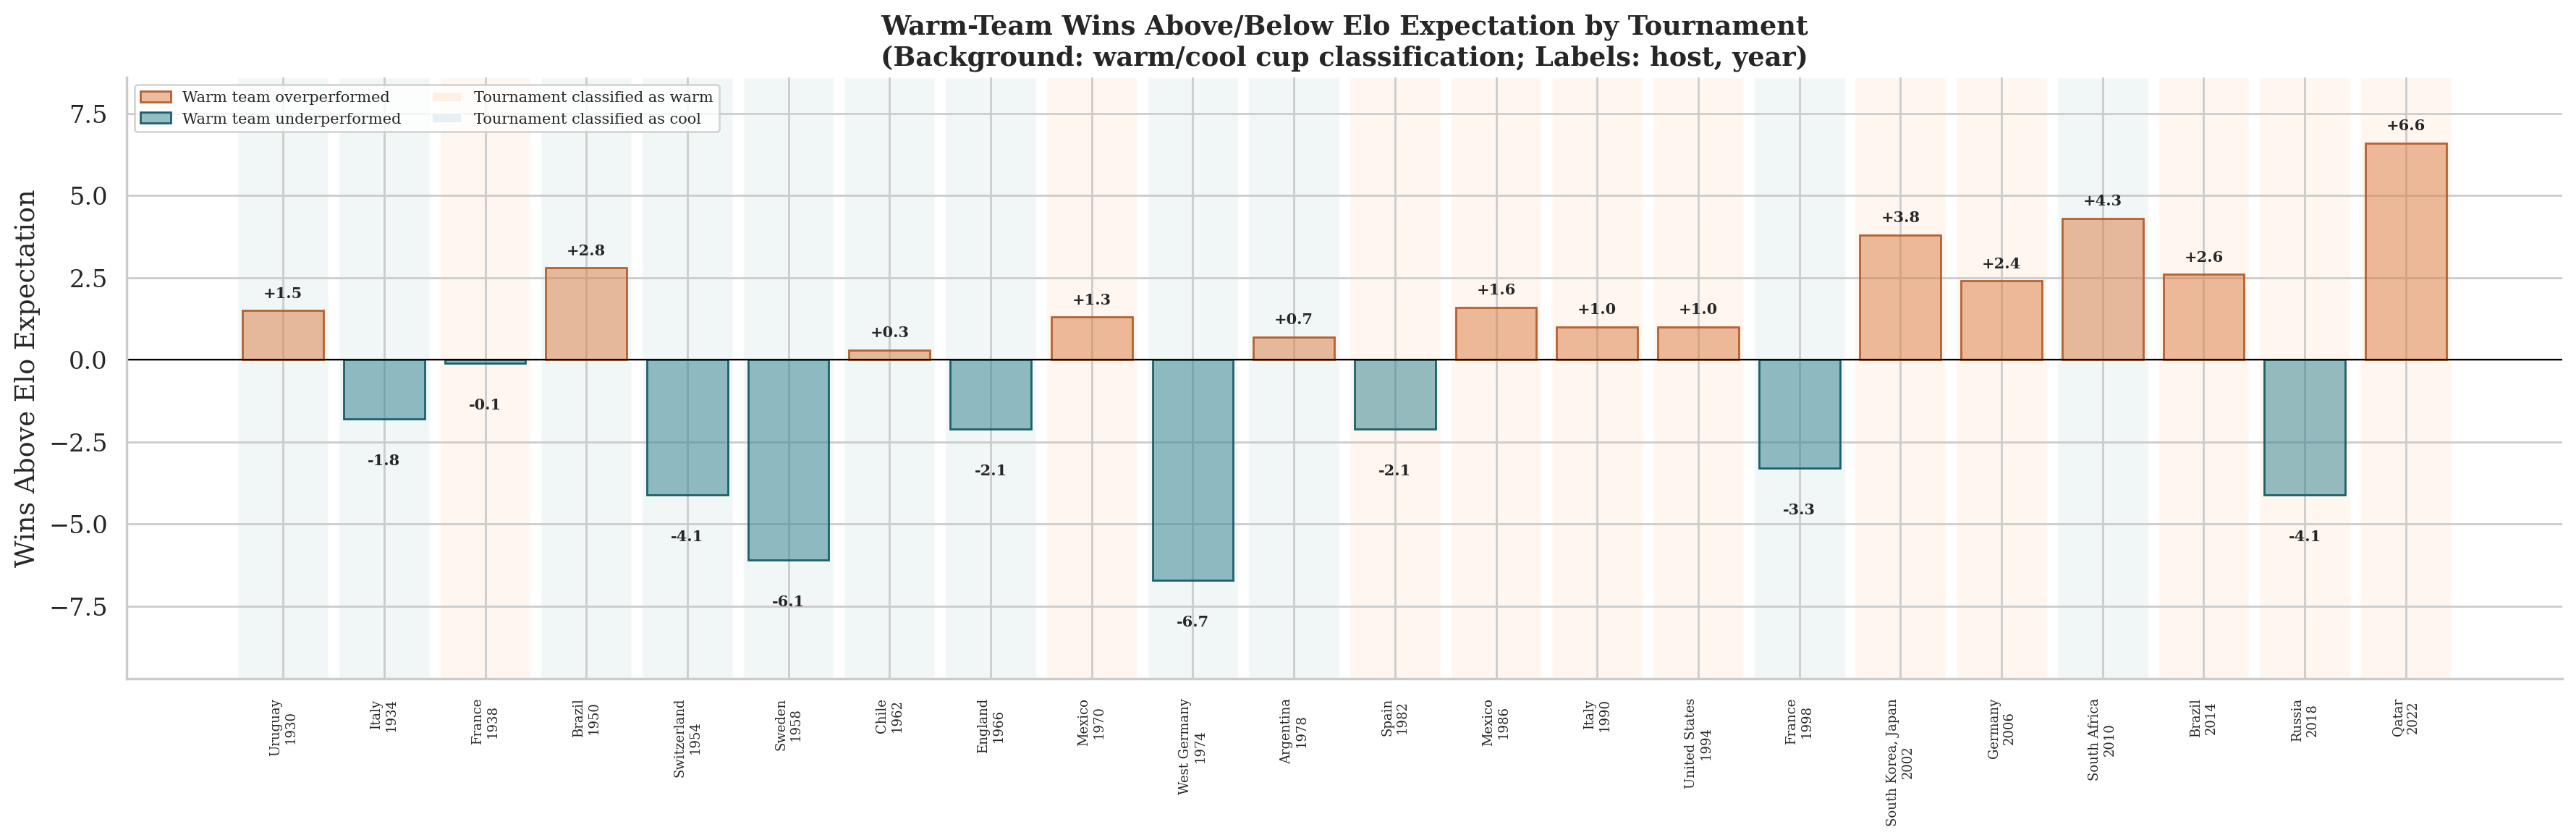
\includegraphics[width=\textwidth]{figures/per_tournament_overperformance.png}
    \caption{Per-tournament warm-team wins above/below Elo expectation. Amber bars indicate overperformance (warm teams exceeded Elo prediction); teal bars indicate underperformance. Values annotated in wins.}
    \label{fig:timeline}
\end{figure}

\subsection{Expected vs Actual Performance}

Figure~\ref{fig:exp_vs_act} decomposes the finding into its components. The left panel shows that warm teams have nearly identical Elo-expected win probabilities in warm cups (0.493) and cool cups (0.499), but their actual performance differs markedly: they achieve 0.519 in warm cups versus 0.469 in cool cups. The right panel shows the cumulative effect: warm teams have won approximately 15 more matches than Elo prediction would expect in warm tournaments, while winning roughly 12 fewer in cool tournaments.

\begin{figure}[H]
    \centering
    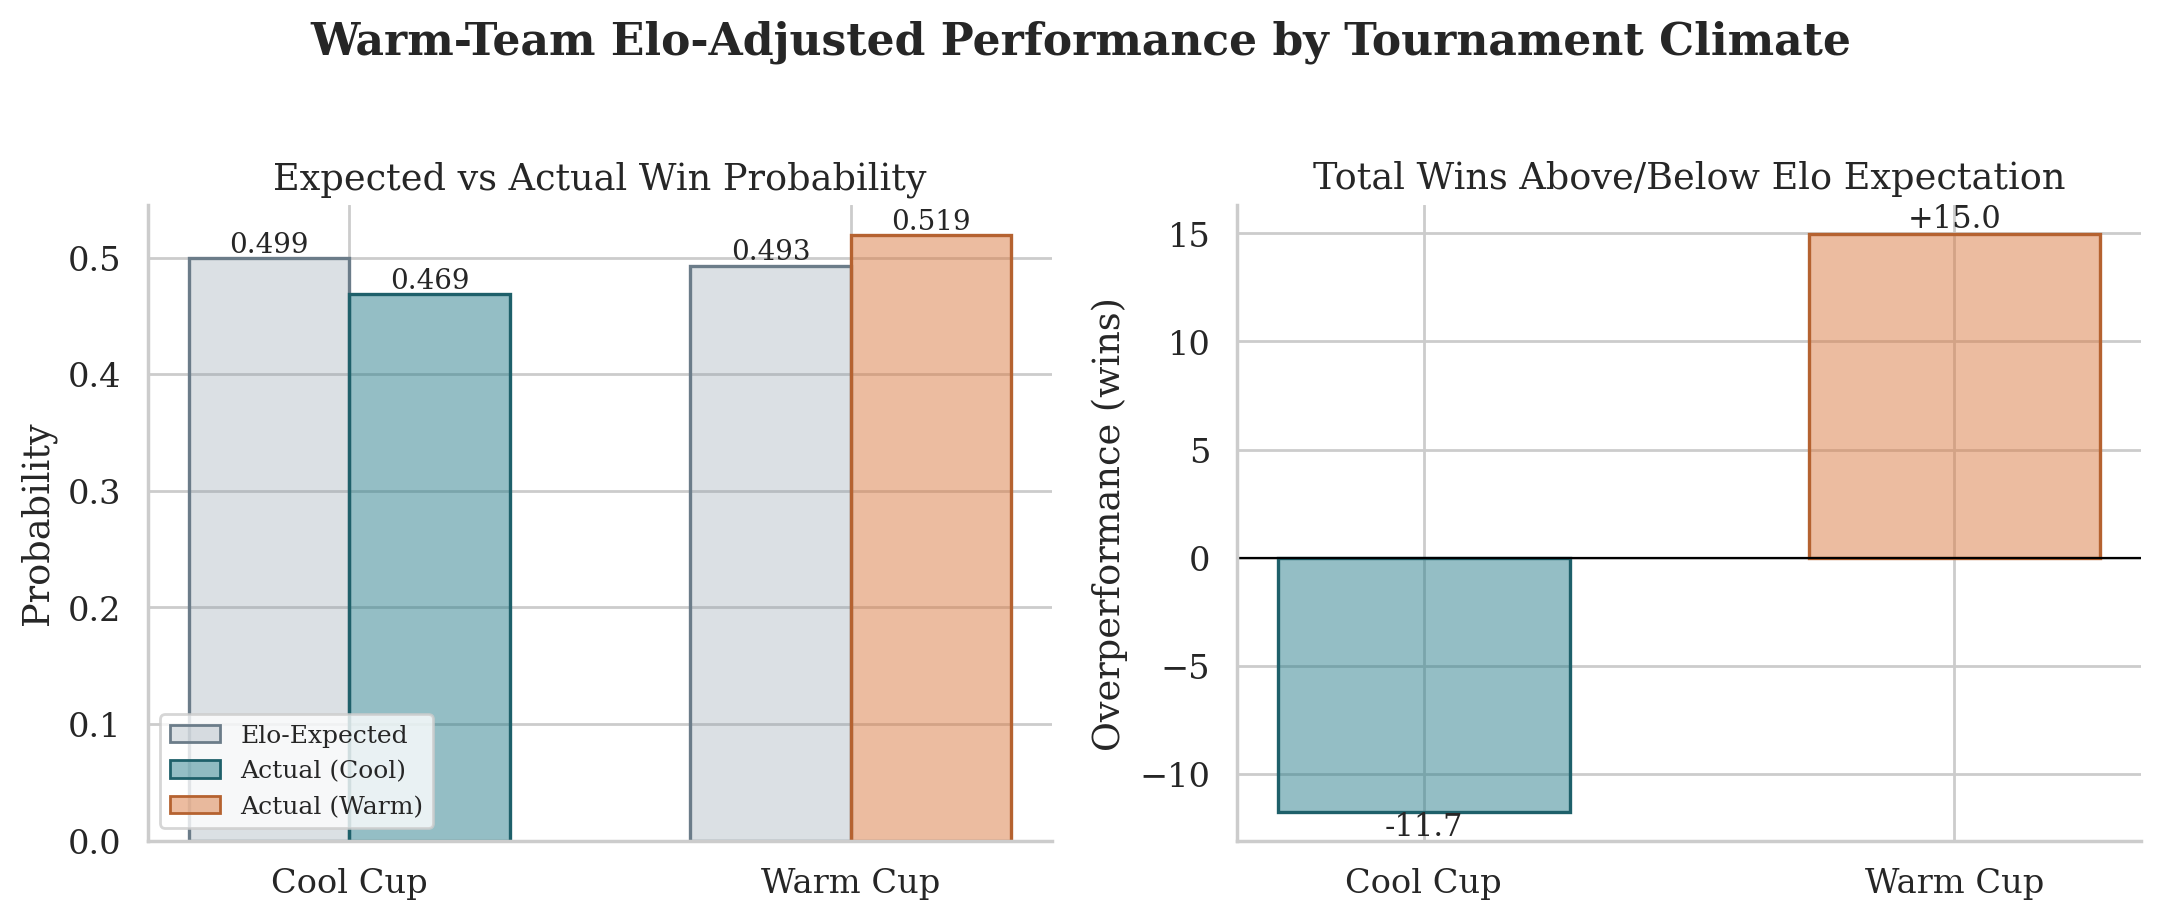
\includegraphics[width=\textwidth]{figures/expected_vs_actual_overperformance.png}
    \caption{Left: Warm-team expected vs actual win probabilities in warm vs cool World Cups. Right: Cumulative wins above/below Elo expectation.}
    \label{fig:exp_vs_act}
\end{figure}

\subsection{Symmetry of the Climate Effect}

The climate effect is not a one-sided warm-team bonus; it is symmetric. Figure~\ref{fig:symmetry} shows the mirror-image pattern: warm-climate teams overperform in warm cups ($+0.026$) and underperform in cool cups ($-0.030$), while cool-climate teams show the exact inverse ($-0.026$ in warm cups, $+0.030$ in cool cups). This symmetry is exactly what one would expect from a genuine climate-driven mechanism rather than a confounded artefact.

\begin{figure}[H]
    \centering
    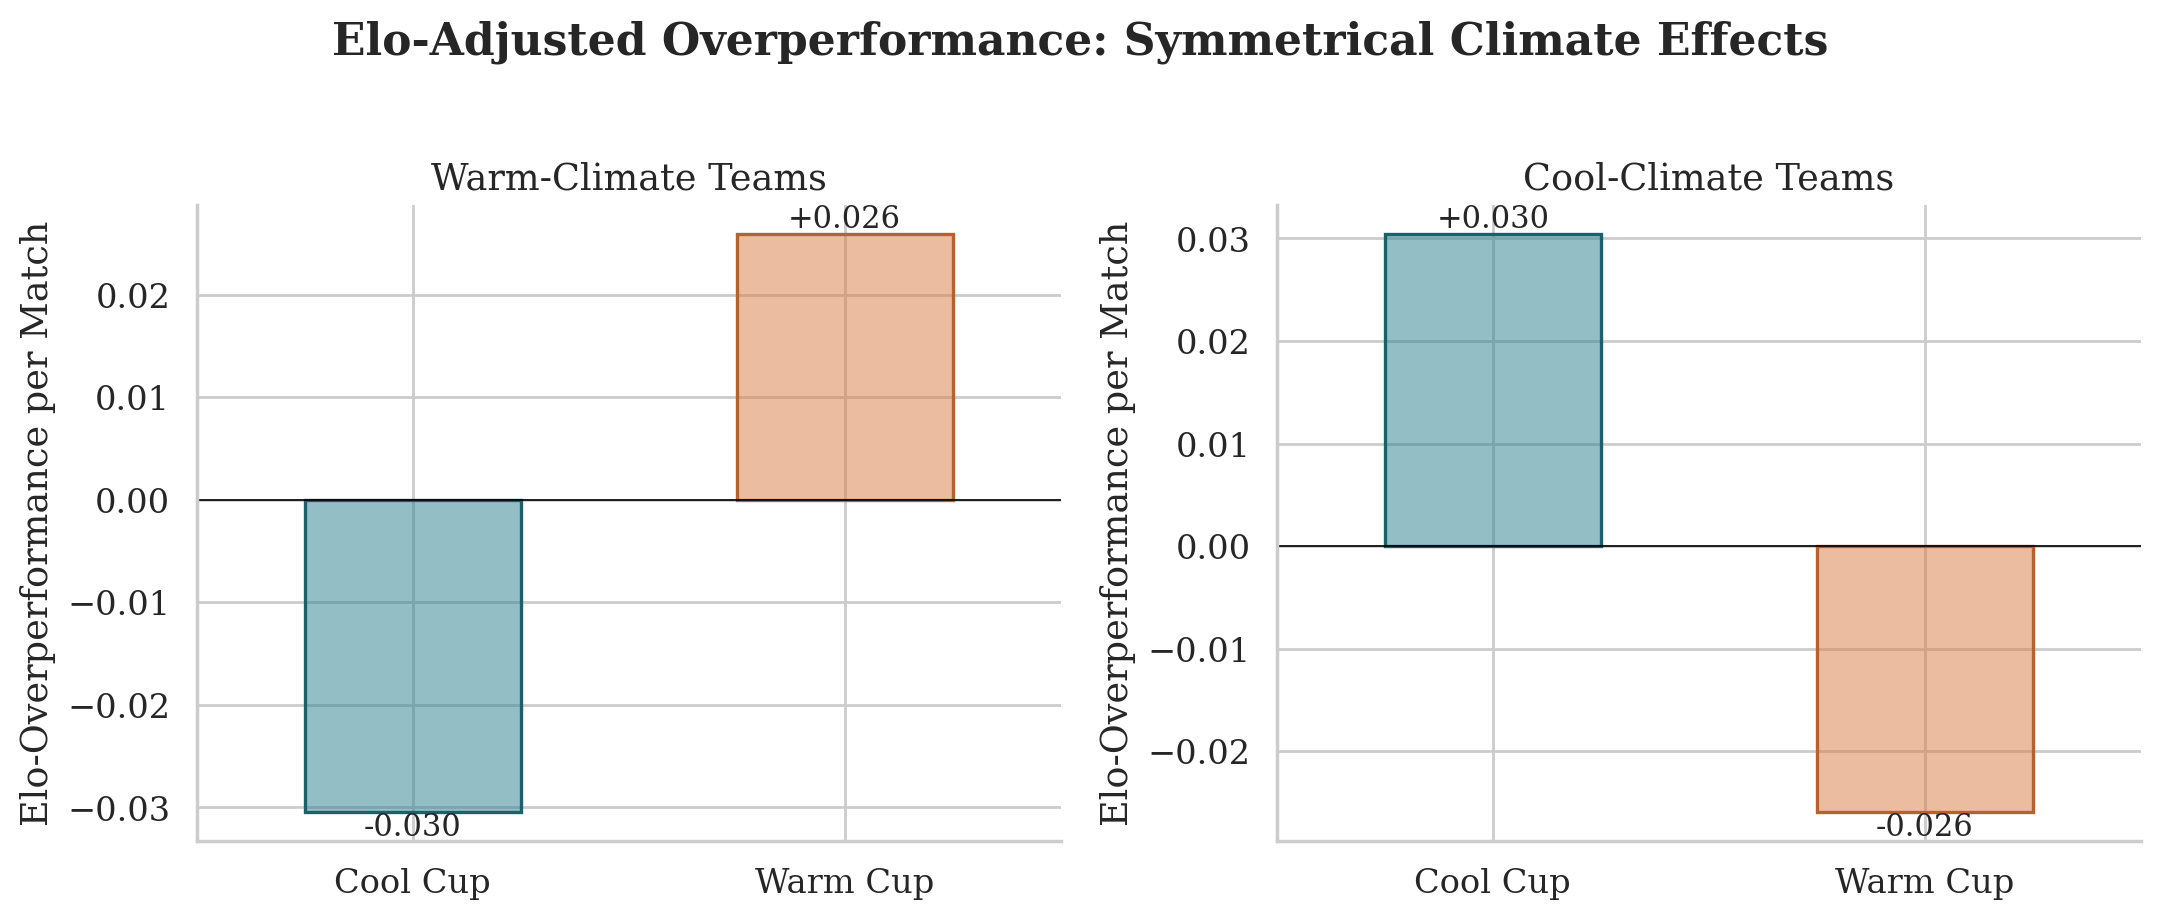
\includegraphics[width=\textwidth]{figures/warm_cool_overperformance_comparison.png}
    \caption{Symmetrical climate effects: warm-climate teams (left) and cool-climate teams (right) show mirror-image Elo-overperformance patterns in warm versus cool World Cups. The magnitudes are nearly identical ($\pm 0.026$--$0.030$), confirming a bidirectional climate mechanism.}
    \label{fig:symmetry}
\end{figure}

\subsection{Robustness Checks}

\textit{Confounding: participation composition.} Warmer tournaments may simply feature more warm-climate teams, creating a mechanical advantage. The proportion of warm-climate teams in each tournament's field is added as a control variable in a multiple regression: $\text{Overperformance} \sim \text{Temperature} + \text{Warm\_Proportion}$. The warm-team proportion is uncorrelated with tournament temperature ($r\approx 0.00$, $p=0.986$), and the temperature coefficient is largely unaffected by its inclusion, confirming that the composition effect does not explain the climate signal.

\textit{Host nation exclusion.} Host nations may benefit from home advantage inflating their performance beyond Elo expectation. All matches involving the designated host nation(s) are flagged and the full analysis is re-run excluding these matches. Figure~\ref{fig:host} confirms that the climate effect direction and magnitude remain consistent whether or not host matches are included. In fact, the gap widens slightly when host matches are excluded ($+0.067$ vs $+0.056$), indicating that host advantage is suppressing rather than inflating the climate signal.

\begin{figure}[H]
    \centering
    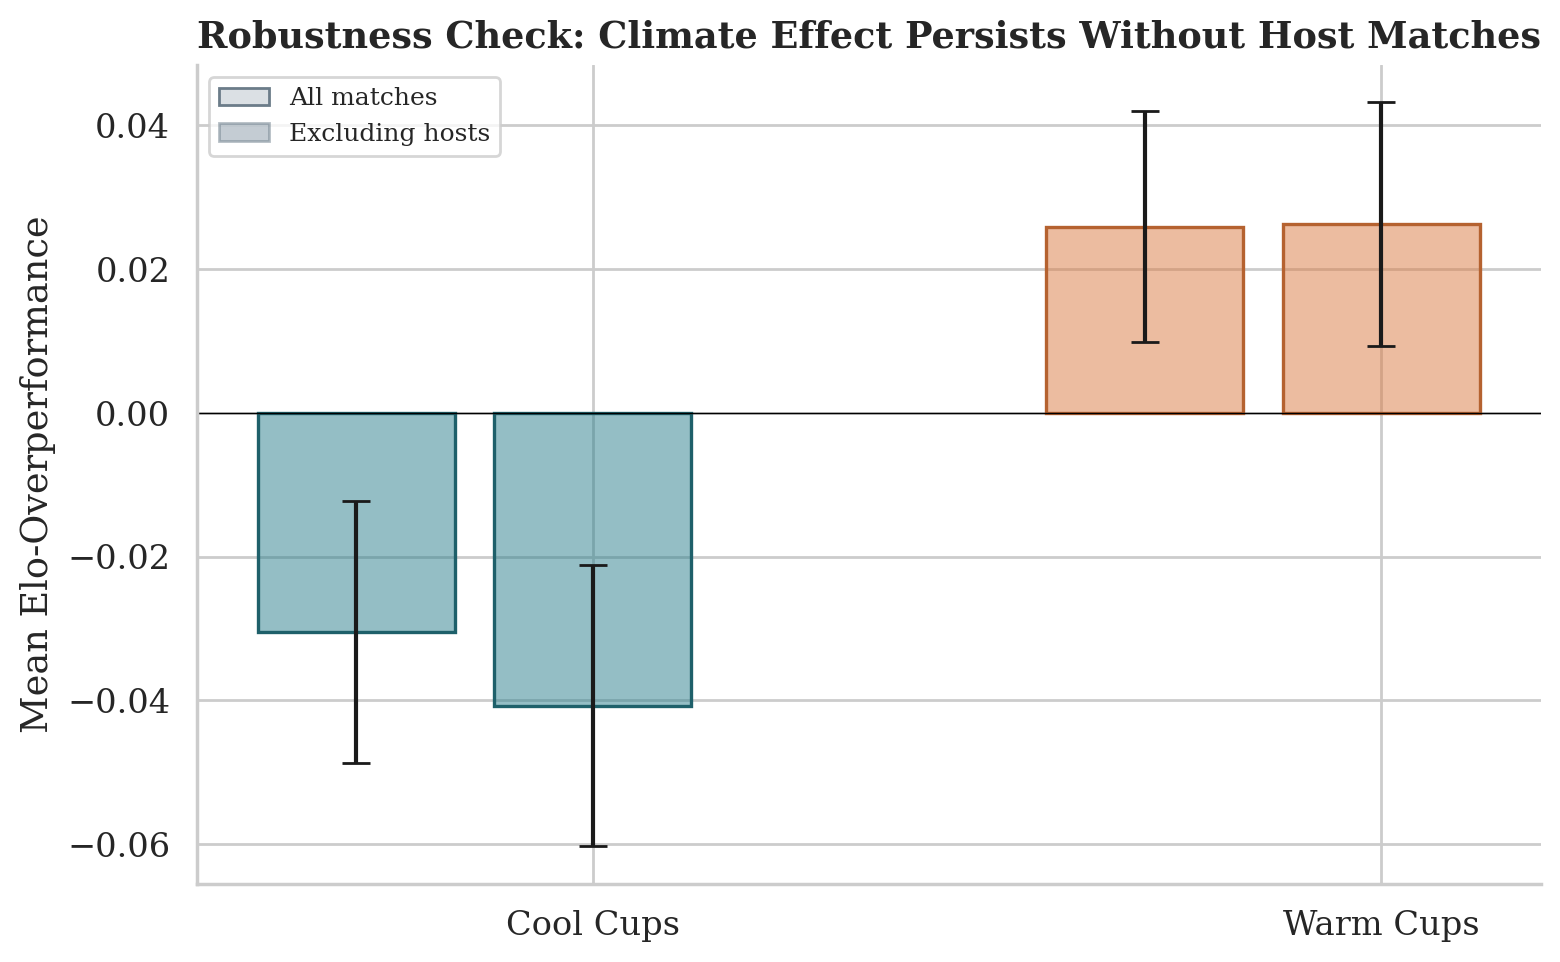
\includegraphics[width=0.8\textwidth]{figures/host_robustness.png}
    \caption{Robustness check: warm-team overperformance in warm vs cool cups, with and without host nation matches. Error bars show $\pm 1$ standard error of the mean. The effect persists and is directionally consistent.}
    \label{fig:host}
\end{figure}

\textit{Threshold sensitivity.} The binary warm/cool classification is sensitive to the specific temperature threshold chosen. Figure~\ref{fig:threshold} presents a full sweep of classification thresholds from $15^{\circ}$C to $25^{\circ}$C. The $t$-statistic exceeds the critical value of $1.96$ for a wide range of thresholds, indicating that the finding is robust to the classification choice and is not an artefact of the specific $19.3^{\circ}$C median split.

\begin{figure}[H]
    \centering
    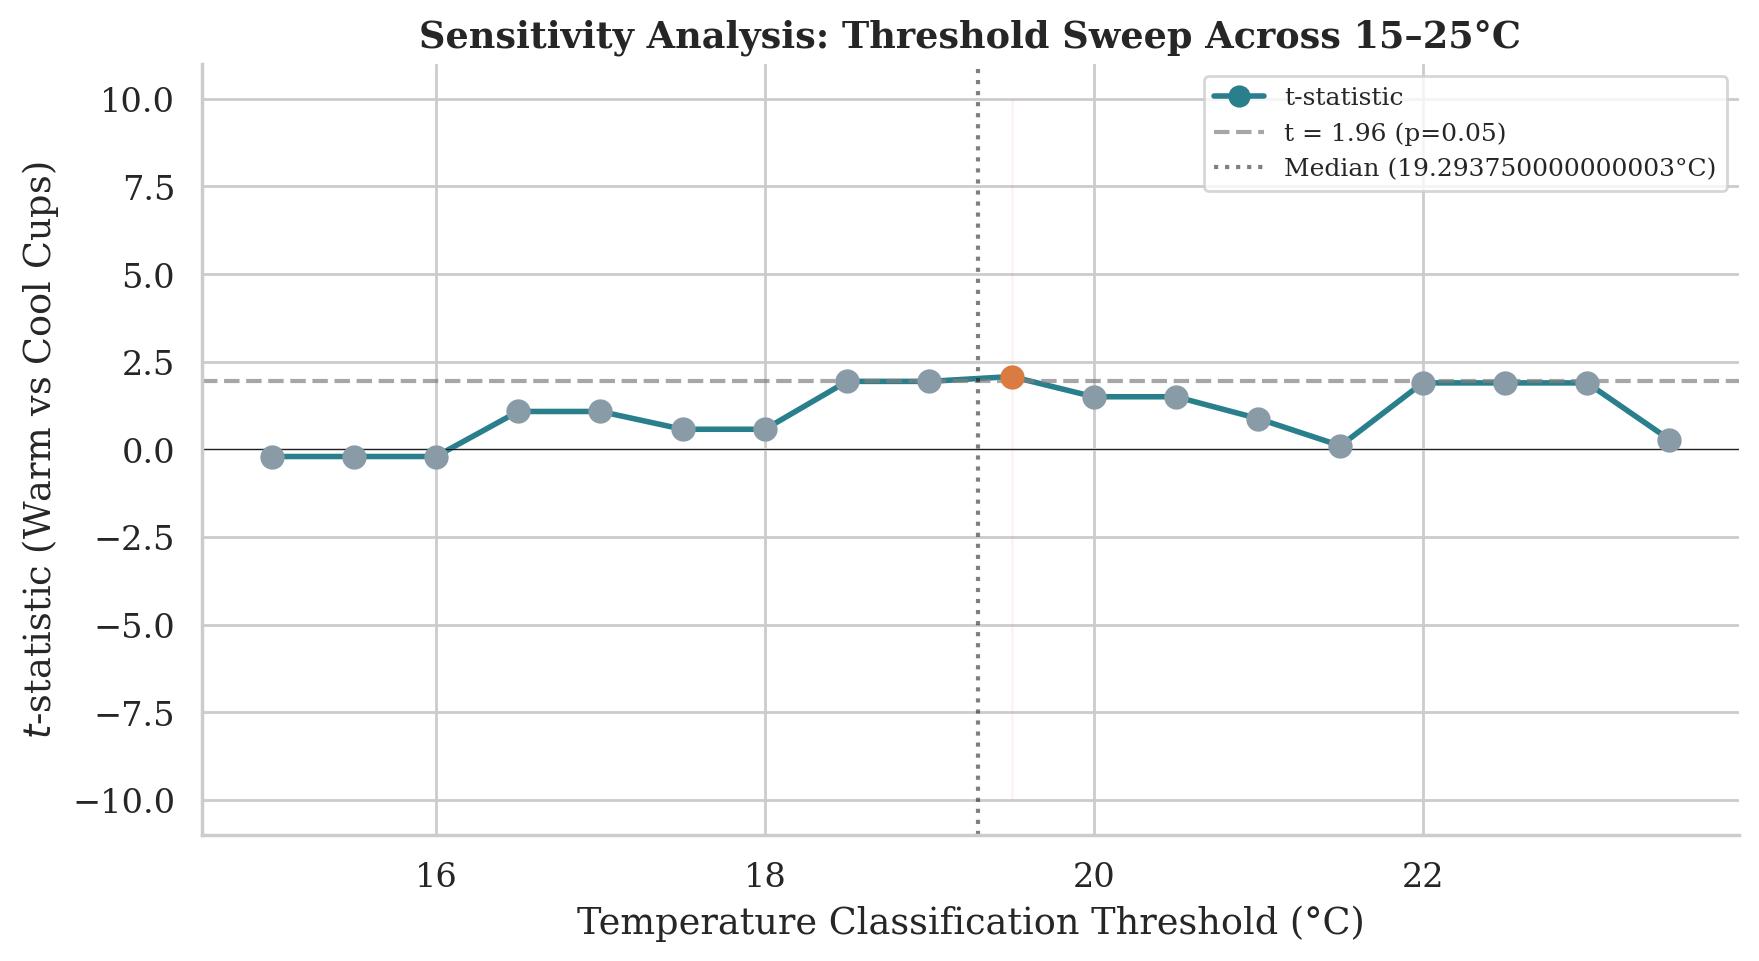
\includegraphics[width=0.9\textwidth]{figures/threshold_sensitivity.png}
    \caption{Sensitivity to temperature classification threshold. The dashed horizontal line marks $t=1.96$ ($p=0.05$). Points in amber indicate thresholds where the warm/cool cup difference is significant. The finding is robust across a broad band of classification thresholds.}
    \label{fig:threshold}
\end{figure}

\subsection{Era Analysis and Mechanism}

Splitting the data into pre-1990 and post-1990 eras reveals an important interpretive nuance. Figure~\ref{fig:era} and Table~\ref{tab:era} present the era-level breakdown. The pre-1990 era shows a larger warm/cool gap ($+0.057$ per match), but this is primarily driven by warm teams being heavily penalised in cool European cups (1954 Switzerland, 1958 Sweden, 1966 England, 1974 West Germany), rather than by a warm-cup bonus. In the post-1990 era, the gap narrows to $+0.029$ per match, and warm teams now roughly break even even in cool cups. This reflects the globalisation of football development: African and Asian teams that were uncompetitive in early tournaments have closed the quality gap.

\begin{figure}[H]
    \centering
    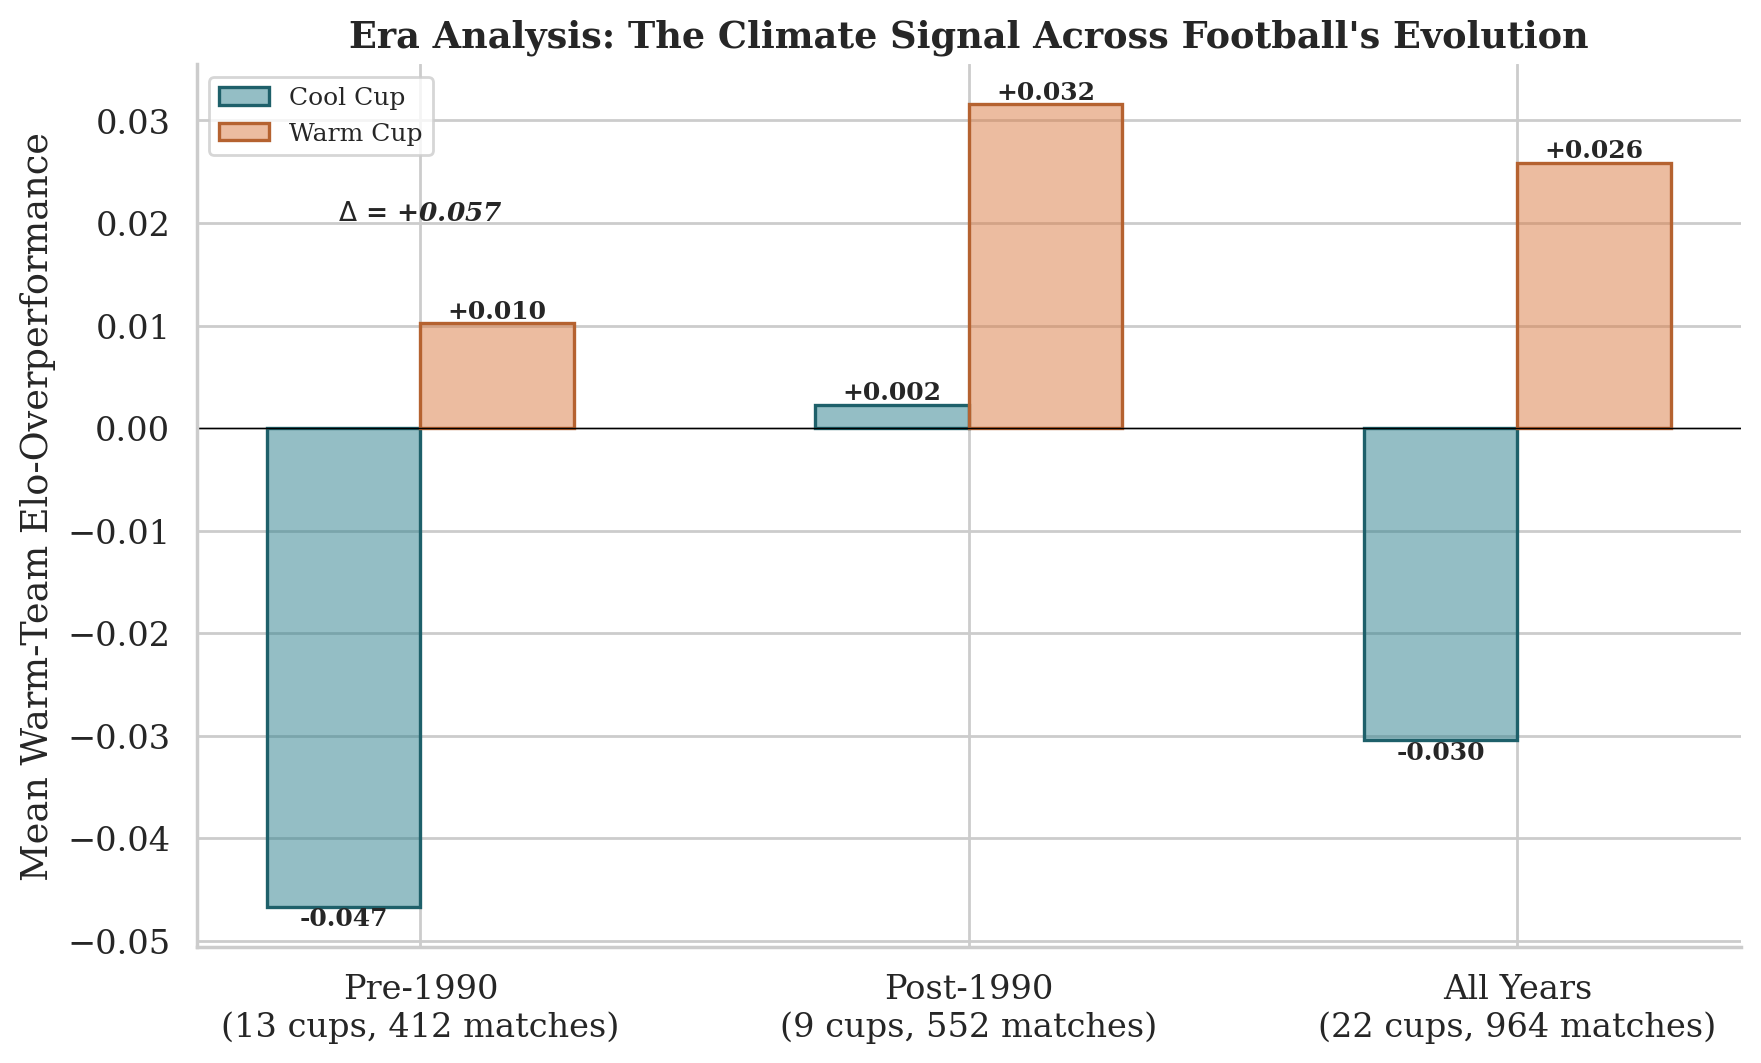
\includegraphics[width=\textwidth]{figures/era_analysis.png}
    \caption{Era analysis of warm-team Elo-overperformance. Pre-1990 (left): large gap driven by severe cool-cup underperformance. Post-1990 (centre): narrower gap, with warm-cup overperformance driving the difference. All years (right): combined $+0.056$ gap.}
    \label{fig:era}
\end{figure}

\begin{table}[H]
    \centering
    \caption{Era-Split Analysis of Warm-Team Overperformance}
    \label{tab:era}
    \begin{tabular}{@{}lcccccc@{}}
        \toprule
        Era & Tournaments & Matches & Warm Cup Mean & Cool Cup Mean & Gap & $t$-test $p$ \\
        \midrule
        Pre-1990 & 13 & 412 & $+0.010$ & $-0.047$ & $+0.057$ & $0.110$ \\
        Post-1990 & 9 & 552 & $+0.032$ & $+0.002$ & $+0.029$ & $0.462$ \\
        All years & 22 & 964 & $+0.026$ & $-0.030$ & $+0.056$ & $0.023$ \\
        \bottomrule
    \end{tabular}
\end{table}

Neither era is independently significant due to reduced sample sizes, but the directions are consistent. The combined finding achieves significance because it pools information across both periods. The post-1990 residual advantage of $+0.032$ in warm cups is the best estimate of the genuine climate effect in modern football, and this figure is used in the predictive section.

\newpage

% ======================================================================
\section{Constructing the Climate Adjustment}
% ======================================================================

The historical analysis provides a per-match climate effect estimate of $\Delta = +0.032$ for warm-climate teams in warm-tournament matches (post-1990 era). This is operationalised as follows.

For any given knockout fixture at the 2026 World Cup, a \textit{climate differential score} is computed between the two teams:

\begin{equation}
    \text{Climate\_Diff\_Score} = (S_{\text{warm}} - S_{\text{cool}}) \times \frac{T_{\text{venue}}}{28^{\circ}\text{C}}
\end{equation}

where $S_{\text{warm}}$ and $S_{\text{cool}}$ are the continuous climate scores for the two teams (derived from K\"{o}ppen codes: Tropical A $=1.0$, Arid Hot BWh/BSh $=0.9$, Temperate C $=0.5$, Cold Arid BWk/BSk $=0.4$, Continental D $=0.2$), and $T_{\text{venue}}$ is the estimated venue temperature for that matchup slot. The denominator of $28^{\circ}$C is chosen as the performance-impairing threshold identified in the exercise physiology literature \citep{chmura2017}. Below $22^{\circ}$C, the Climate\_Diff\_Score is set to zero; below this threshold, heat stress is not expected to meaningfully impair performance.

The per-match win probability adjustment for Approach~1 (post-hoc flagging) is then:

\begin{equation}
    p_{\text{adjust}} = \Delta \times \text{Climate\_Diff\_Score}
\end{equation}

For Approach~2 (climate-adjusted simulation), the adjustment is applied to the warm team's goal-scoring Poisson parameter as a multiplier $1 + \min(0.10,\; 3 \times \Delta \times \text{Climate\_Diff\_Score})$, with the cool team receiving the inverse adjustment. This embeds the climate effect directly into the match simulation dynamics.

\newpage

% ======================================================================
\section{2026 Predictive Model}
% ======================================================================

\subsection{Setup}

The 2026 World Cup features 48 teams across 12 groups of 4, with the top two from each group plus the eight best third-place teams advancing to a 32-team knockout bracket. The complete group-stage fixture list (72 matches) is constructed from Wikipedia, with each match assigned to a specific host city. The knockout bracket is based on the official FIFA bracket structure, including the full third-place team allocation table (495 cases) that determines which R32 slot each qualifying third-place team occupies.

Each of the 48 teams is assigned a current Elo rating computed through June 2026 using the same methodology as the historical analysis. These ratings serve as the baseline for the Monte Carlo simulation. The tournament is contextually warm ($22.6^{\circ}$C average, above the 19.3$^{\circ}$C historical median). The climate adjustment is applied per-match rather than tournament-wide: climate effects are triggered only when an individual knockout fixture pairs a warm-climate team against a cool-climate team and the pre-assigned venue temperature exceeds a relevant threshold. The two approaches below operationalise this differently: both approaches use a 22.0$^{\circ}$C venue temperature threshold: Approach~1 applies it for post-hoc flagging of warm-venue climate clashes, while Approach~2 uses it as the activation point for in-simulation goal-expectation adjustment.

\subsection{Approach 1: Post-Hoc Climate Flagging on a Clean Elo Simulation}

The simulation runs 100,000 independent full-tournament Monte Carlo simulations using a Poisson goal model calibrated to historical World Cup averages (home 1.77, away 1.05 goals per match). The Elo update function uses a smart K-factor that scales down for group-stage matches ($\times 0.5$) and scales up for knockout rounds ($\times 2.0$ for the final), with a parity multiplier that increases K for evenly matched teams and decreases it for mismatches, and an upset bonus ($\times 1.5$) for underdog wins.

The simulation tracks every pairwise encounter across all knockout rounds, producing a $48\times48$ matchup probability matrix. The climate adjustment is then overlaid as a post-hoc flag on every warm-versus-cool matchup.

\subsubsection{Climate Flag Tiers}
For each of the 1,024 possible knockout matchups, the climate differential score is computed between the two teams weighted by the estimated venue temperature. Matchups are classified into three tiers:

\begin{itemize}[leftmargin=*]
    \item \textbf{Tier 1 (Strong):} Climate\_Diff\_Score $> 0.20$ AND Matchup Probability $\geq 7\%$
    \item \textbf{Tier 2 (Moderate):} Climate\_Diff\_Score $> 0.10$ AND Matchup Probability $\geq 3\%$
    \item \textbf{Tier 3 (Weak):} Climate clash ($\text{Warm} \neq \text{Cool}$) but below the above thresholds
\end{itemize}

Of the 1,024 possible knockout matchups, 484 are warm-versus-cool clashes, of which 229 occur in warm-venue conditions (venue temperature $>22^{\circ}$C). Ten matchups receive Tier~1 flags and 27 receive Tier~2 flags.

Figure~\ref{fig:scatter} presents the headline visualisation: all warm-venue climate clashes plotted as matchup probability against Elo difference, with Tier~1, Tier~2, and Tier~3 matchups colour-coded.

\begin{figure}[H]
    \centering
    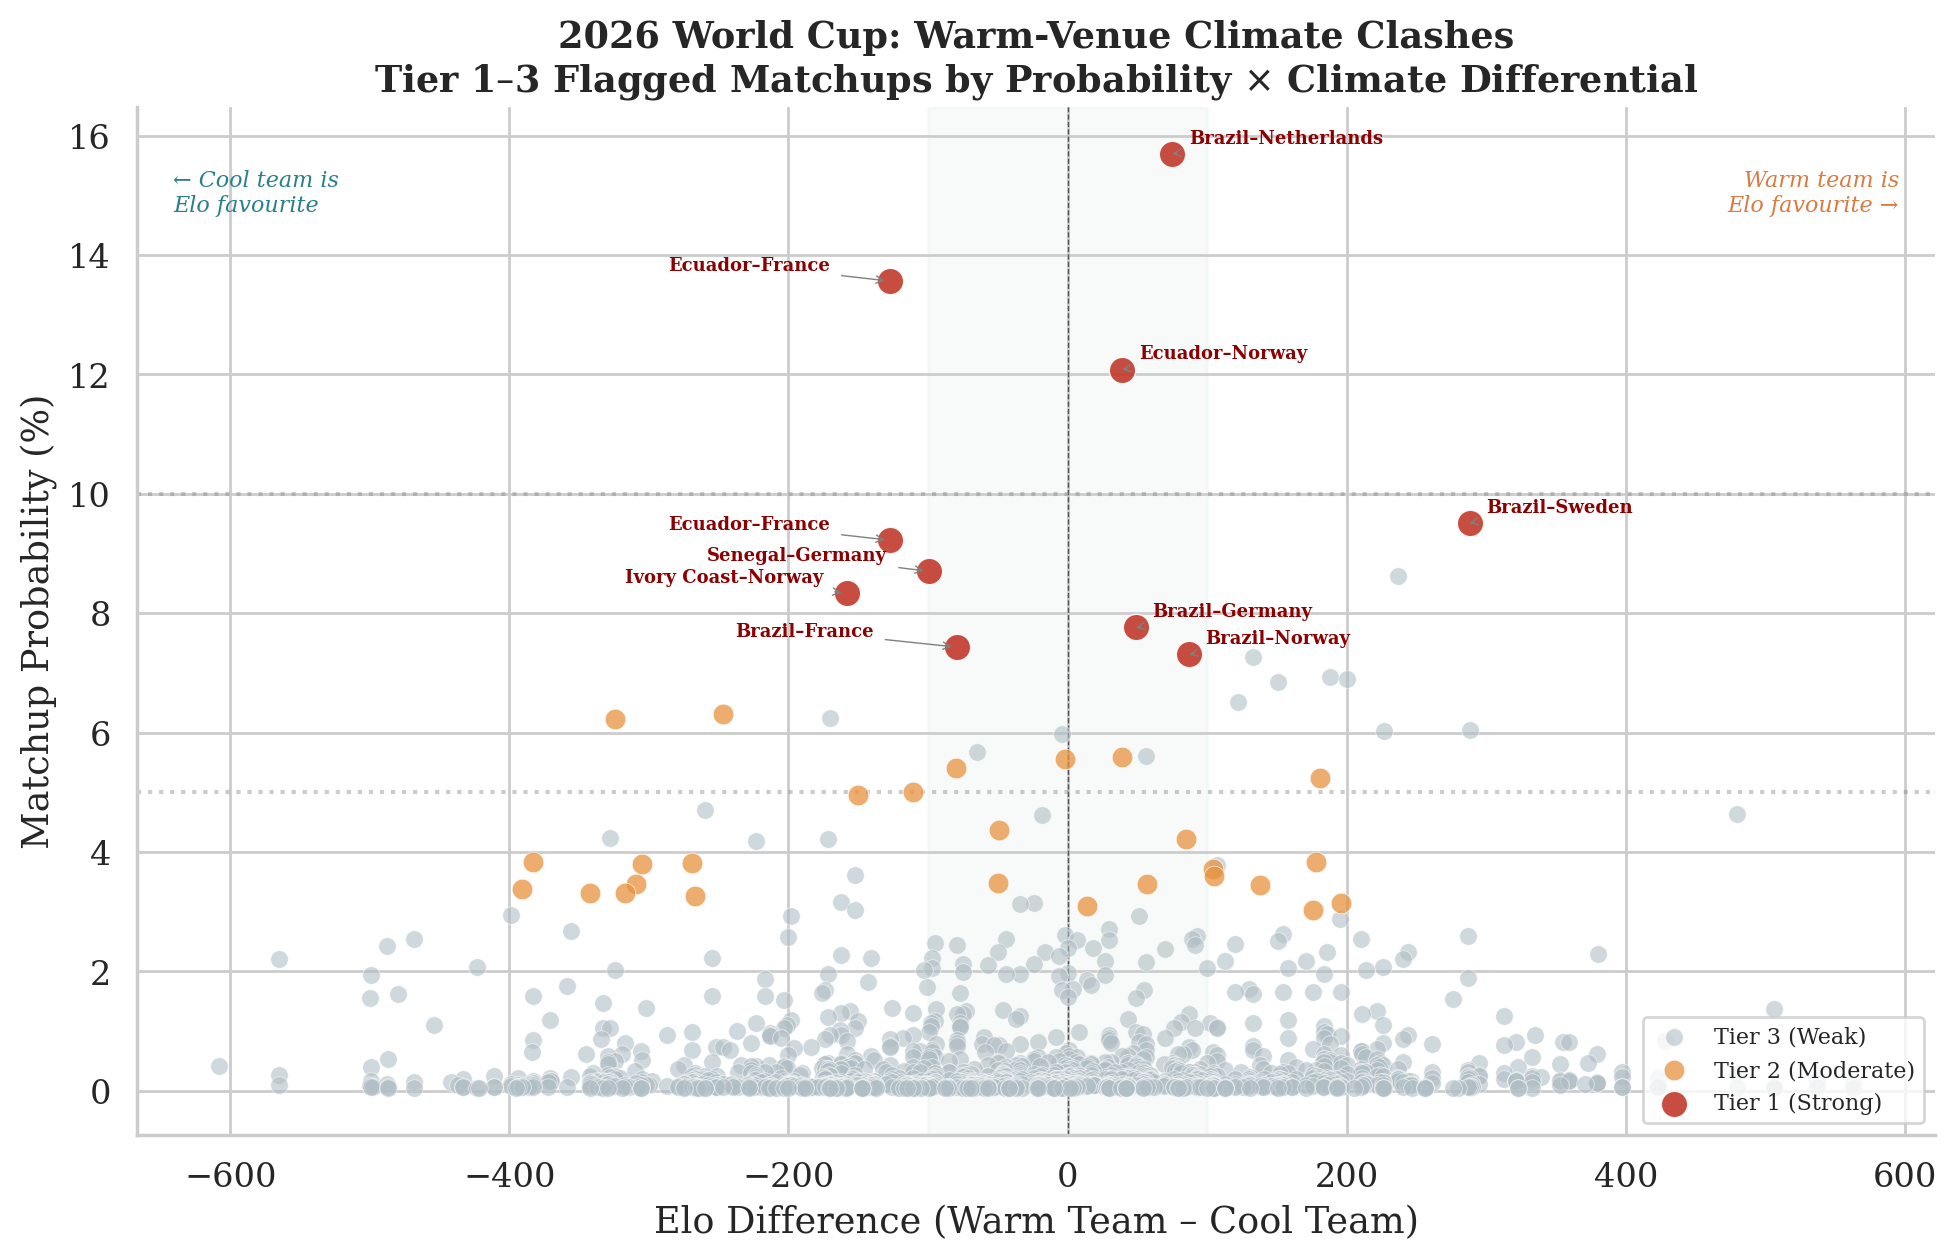
\includegraphics[width=\textwidth]{figures/climate_clash_scatter.png}
     \caption{Warm-venue climate clashes: matchup probability versus Elo difference (warm team minus cool team). Deep red points are Tier 1 (Strong), amber are Tier 2 (Moderate), slate are Tier 3 (Weak). The top Tier 1 matchups are labelled.}
    \label{fig:scatter}
\end{figure}

Table~\ref{tab:flags} presents the top 10 Tier~1 and top 5 Tier~2 flagged matchups, ranked by probability of occurrence.

\begin{table}[H]
    \centering
    \caption{Top Climate-Flagged Knockout Matchups (2026 World Cup)}
    \label{tab:flags}
    \begin{tabular}{@{}llcccc@{}}
        \toprule
        Tier & Warm Team & Cool Team & Probability & Venue Temp & Diff Score & Elo Diff \\
        \midrule
        1 & Brazil & Netherlands & 15.7\% & 28.8$^{\circ}$C & 0.514 & $+75$ \\
        1 & Ecuador & France & 13.6\% & 23.0$^{\circ}$C & 0.411 & $-127$ \\
        1 & Ecuador & Norway & 12.1\% & 22.5$^{\circ}$C & 0.643 & $+39$ \\
        1 & Brazil & Sweden & 9.5\% & 28.8$^{\circ}$C & 0.823 & $+288$ \\
        1 & Ecuador & France & 9.2\% & 22.5$^{\circ}$C & 0.402 & $-127$ \\
        1 & Senegal & Germany & 8.7\% & 22.5$^{\circ}$C & 0.321 & $-99$ \\
        1 & Ivory Coast & Norway & 8.3\% & 22.5$^{\circ}$C & 0.643 & $-158$ \\
        1 & Brazil & Germany & 7.8\% & 22.5$^{\circ}$C & 0.402 & $+49$ \\
        1 & Brazil & France & 7.4\% & 22.5$^{\circ}$C & 0.402 & $-79$ \\
        1 & Brazil & Norway & 7.3\% & 22.5$^{\circ}$C & 0.643 & $+87$ \\
        \midrule
        2 & Ivory Coast & England & 6.3\% & 25.4$^{\circ}$C & 0.454 & $-247$ \\
        2 & Ivory Coast & France & 6.2\% & 22.5$^{\circ}$C & 0.402 & $-324$ \\
        2 & Brazil & England & 5.6\% & 28.0$^{\circ}$C & 0.500 & $-2$ \\
        2 & Tunisia & Scotland & 5.4\% & 28.8$^{\circ}$C & 0.411 & $-80$ \\
        2 & Senegal & Germany & 5.1\% & 25.4$^{\circ}$C & 0.258 & $-99$ \\
        \bottomrule
    \end{tabular}
\end{table}

Brazil--Netherlands (15.7\% probability, climate differential of 0.514 at Guadalupe, 28.8$^{\circ}$C) and Ecuador--France (13.6\%, 0.411 at Miami Gardens, 23.0$^{\circ}$C) are the most likely Tier~1 matchups. Ecuador--France is especially notable: Ecuador are the Elo underdog ($-127$) but the climate differential of 0.411 favouring warm-climate Ecuador over cool-climate France represents a case where the climate effect may offset a quality gap. Brazil--Sweden (9.5\%, 0.823) achieves the highest climate differential of any matchup, though its occurrence probability is lower. Among Tier~2, Ivory Coast--England (6.3\%, 0.454) and Ivory Coast--France (6.2\%, 0.402) show large Elo deficits ($-247$ and $-324$) accompanied by substantial climate differentials, making them the most dramatic potential climate-upset scenarios in the tournament.

\subsubsection{Team-Level Climate Exposure}

Figure~\ref{fig:exposure} ranks teams by their expected climate clash count: the sum of Tier 1 and Tier 2 flagged matchup probabilities across all possible knockout encounters. Values above 1.0 indicate a team can expect more than one climate-flagged clash per tournament run on average.

\begin{figure}[H]
    \centering
    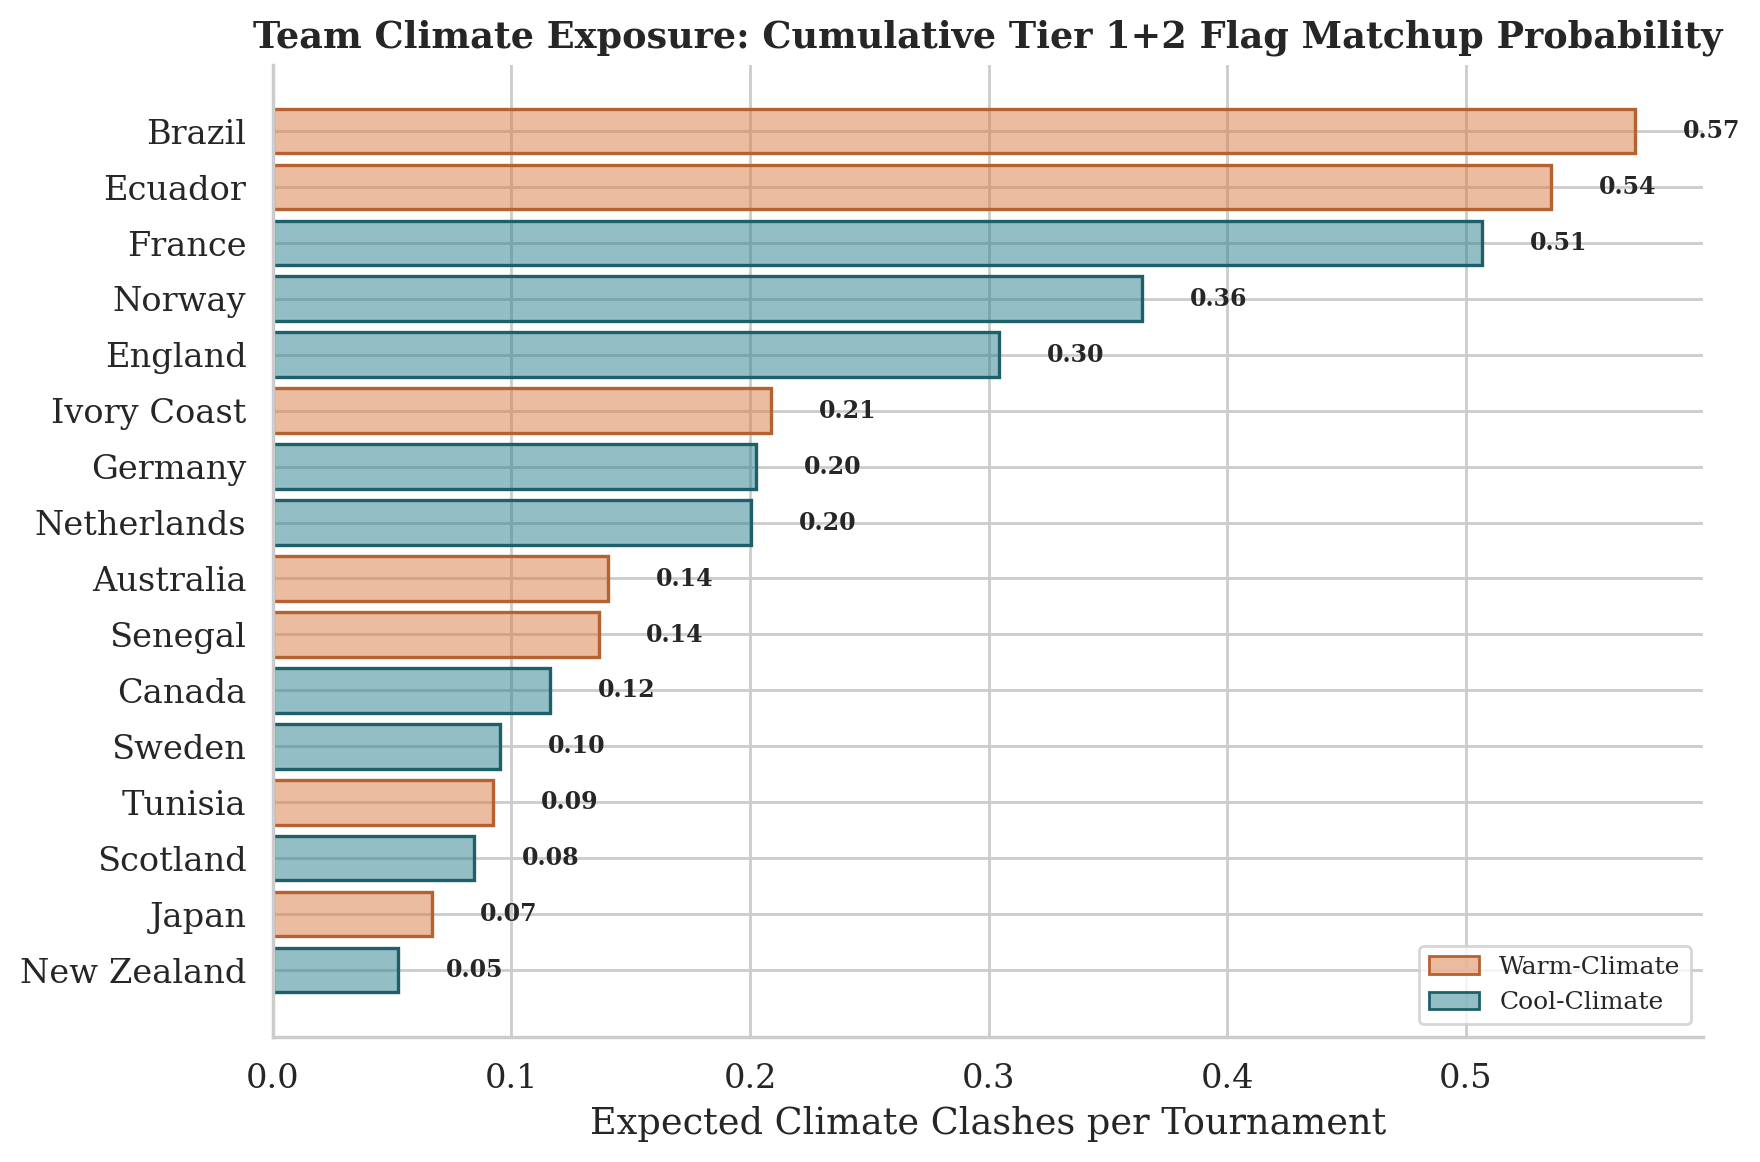
\includegraphics[width=0.85\textwidth]{figures/team_climate_exposure.png}
    \caption{Team climate exposure: expected count of Tier 1 and Tier 2 flagged matchups for the top 16 most-exposed teams. Amber bars indicate warm-climate teams; teal bars indicate cool-climate teams.}
    \label{fig:exposure}
\end{figure}

Table~\ref{tab:exposure} ranks teams by their expected number of climate-flagged clashes.

\begin{table}[H]
    \centering
    \caption{Top 10 Teams by Expected Climate Clashes}
    \label{tab:exposure}
    \begin{tabular}{@{}llc@{}}
        \toprule
        Team & Climate & Expected Clashes \\
        \midrule
        Brazil       & Warm & 0.57 \\
        Ecuador      & Warm & 0.54 \\
        France       & Cool & 0.51 \\
        Norway       & Cool & 0.36 \\
        England      & Cool & 0.30 \\
        Ivory Coast  & Warm & 0.21 \\
        Germany      & Cool & 0.20 \\
        Netherlands  & Cool & 0.20 \\
        Australia    & Warm & 0.14 \\
        Senegal      & Warm & 0.14 \\
        \bottomrule
    \end{tabular}
    \vspace{4pt}
    \par\footnotesize Values represent the expected number of Tier~1+2 climate-flagged matchups per tournament run, summed across all knockout rounds. A value below 1.0 indicates that, on average, fewer than one such matchup is expected per tournament. These are not probabilities and are not capped at 100\%.
\end{table}

The exposure is led by Brazil (0.57 expected climate clashes per tournament run) and Ecuador (0.54), reflecting their high Elo ratings and warm-climate classification making them likely to meet cool-climate opponents in warm knockout venues. France (0.51) has the highest exposure among cool-climate teams, while Norway (0.36) and England (0.30) follow. The climate exposure is spread across roughly the top 10 teams, reflecting the depth of the modern tournament field. No team exceeds an expected value of 1.0, indicating that climate-flagged clashes are relatively rare events even for the most exposed teams.

\subsection{Approach 2: Climate-Adjusted Monte Carlo Simulation}

As an orthogonal validation, a second set of 100,000 full-tournament simulations is run where the climate adjustment is applied \textit{during} each knockout match, rather than as a post-hoc flag. In this approach, whenever a warm-climate team faces a cool-climate team in a knockout match with venue temperature exceeding $22^{\circ}$C, the warm team's goal-scoring Poisson parameter receives a boost proportional to the climate differential score (capped at $+10\%$), and the cool team's parameter receives a corresponding reduction. This embeds the climate mechanism directly into the simulation dynamics rather than layering it on top.

Figure~\ref{fig:approach_winners} compares the tournament win probabilities for the top 20 teams by Elo between the pure-Elo baseline (Approach 1) and the climate-adjusted simulation (Approach 2).

\begin{figure}[H]
    \centering
    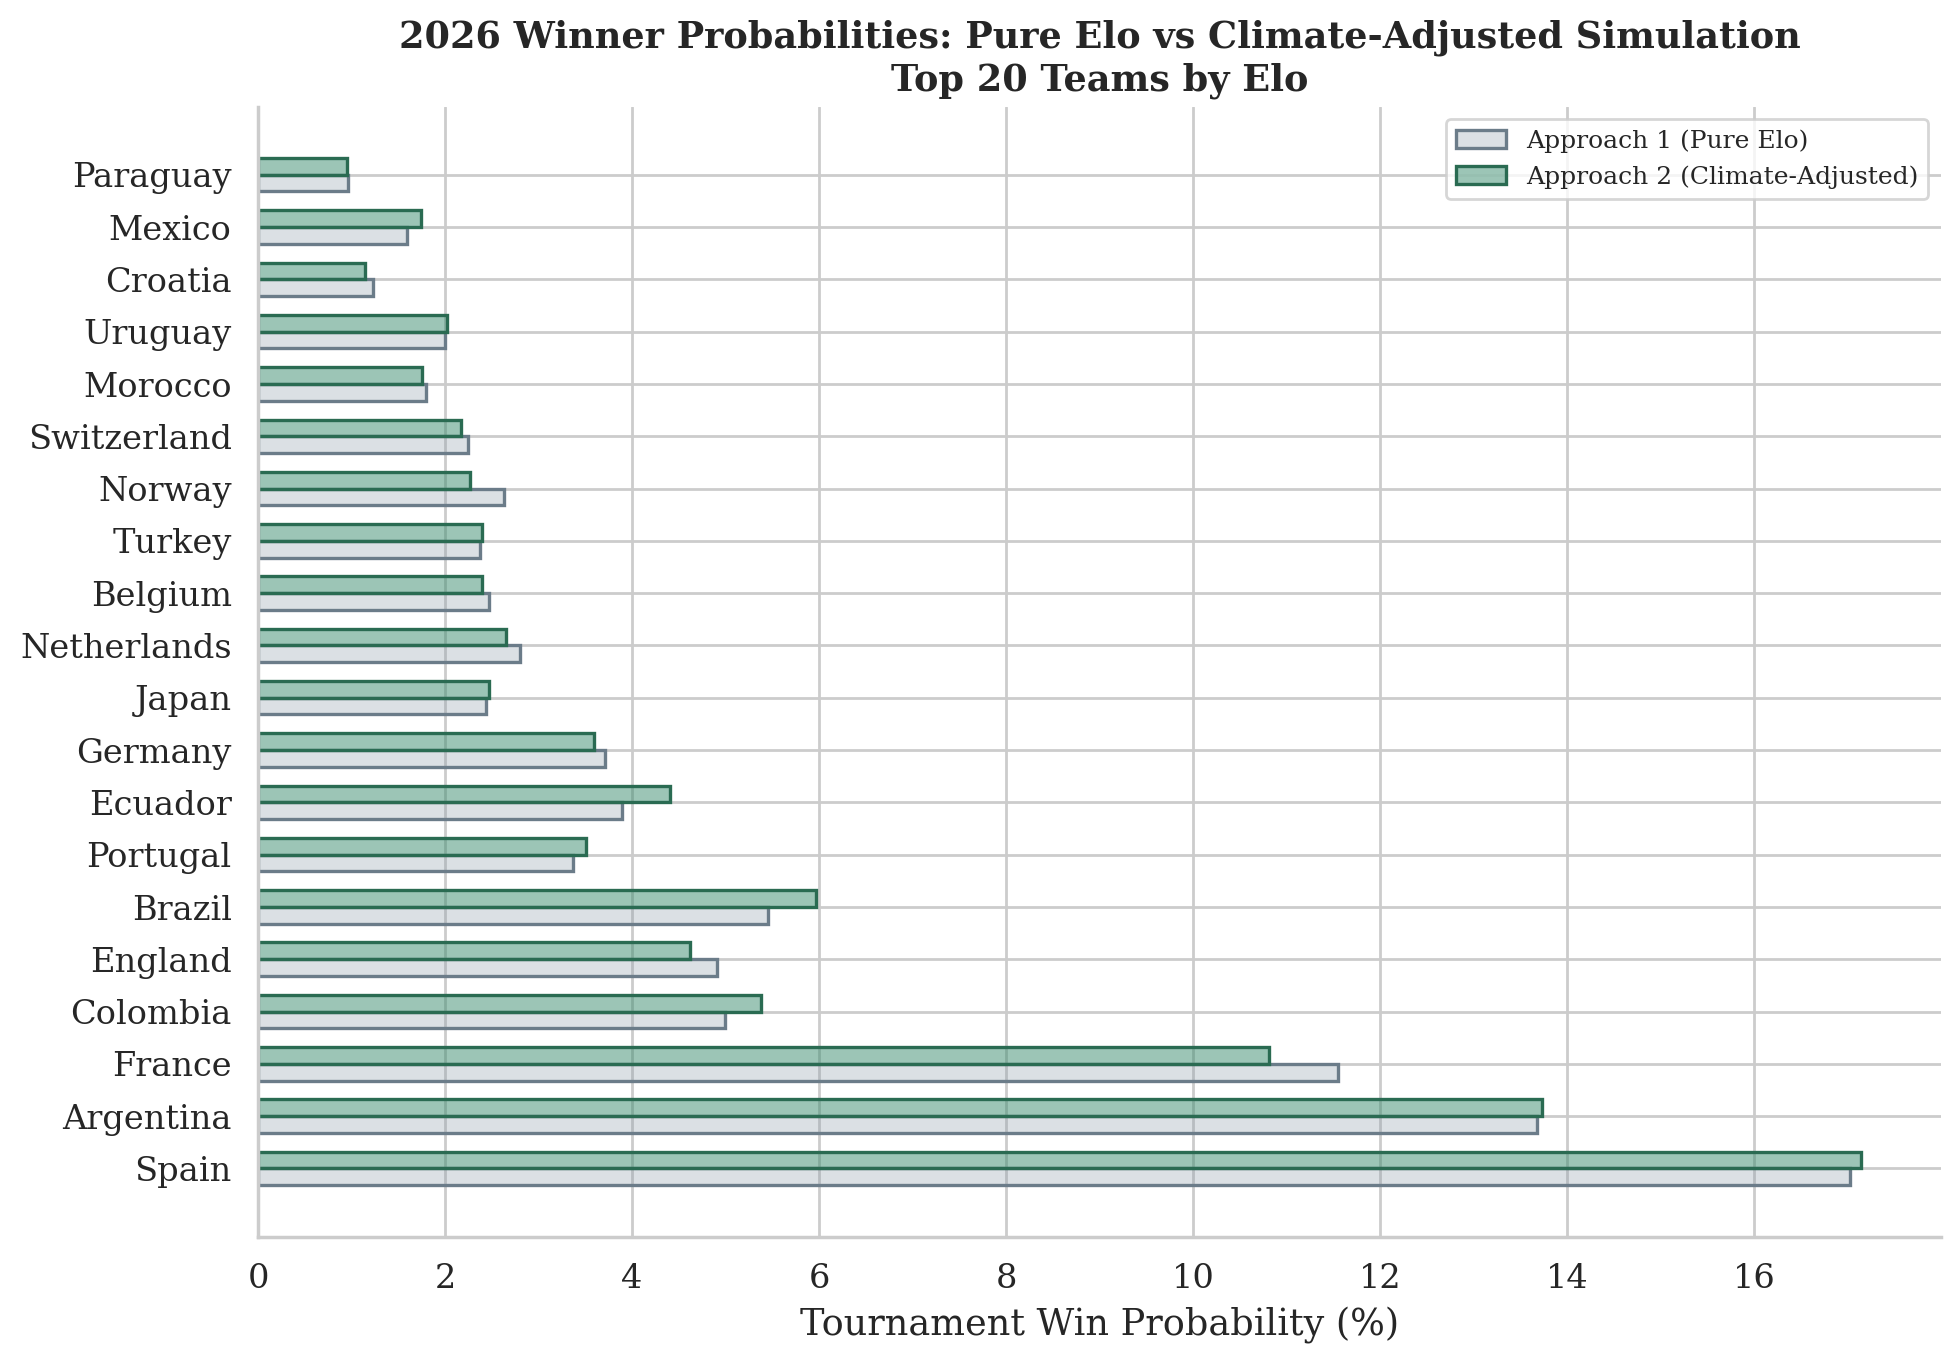
\includegraphics[width=\textwidth]{figures/approach_comparison_winners.png}
     \caption{2026 World Cup winner probabilities: Approach 1 (pure Elo, grey) vs Approach 2 (climate-adjusted, green). Top 20 teams by Elo rating. The bars are nearly indistinguishable at this scale, reflecting the modest magnitude of the climate effect at the tournament level.}
    \label{fig:approach_winners}
\end{figure}

The climate adjustment produces systematic and directional effects. Warm-climate teams gain probability mass; cool-climate teams lose probability mass. Figure~\ref{fig:approach_delta} isolates the win probability deltas, showing the 15 biggest beneficiaries and the 15 teams most disadvantaged by the climate adjustment.

\begin{figure}[H]
    \centering
    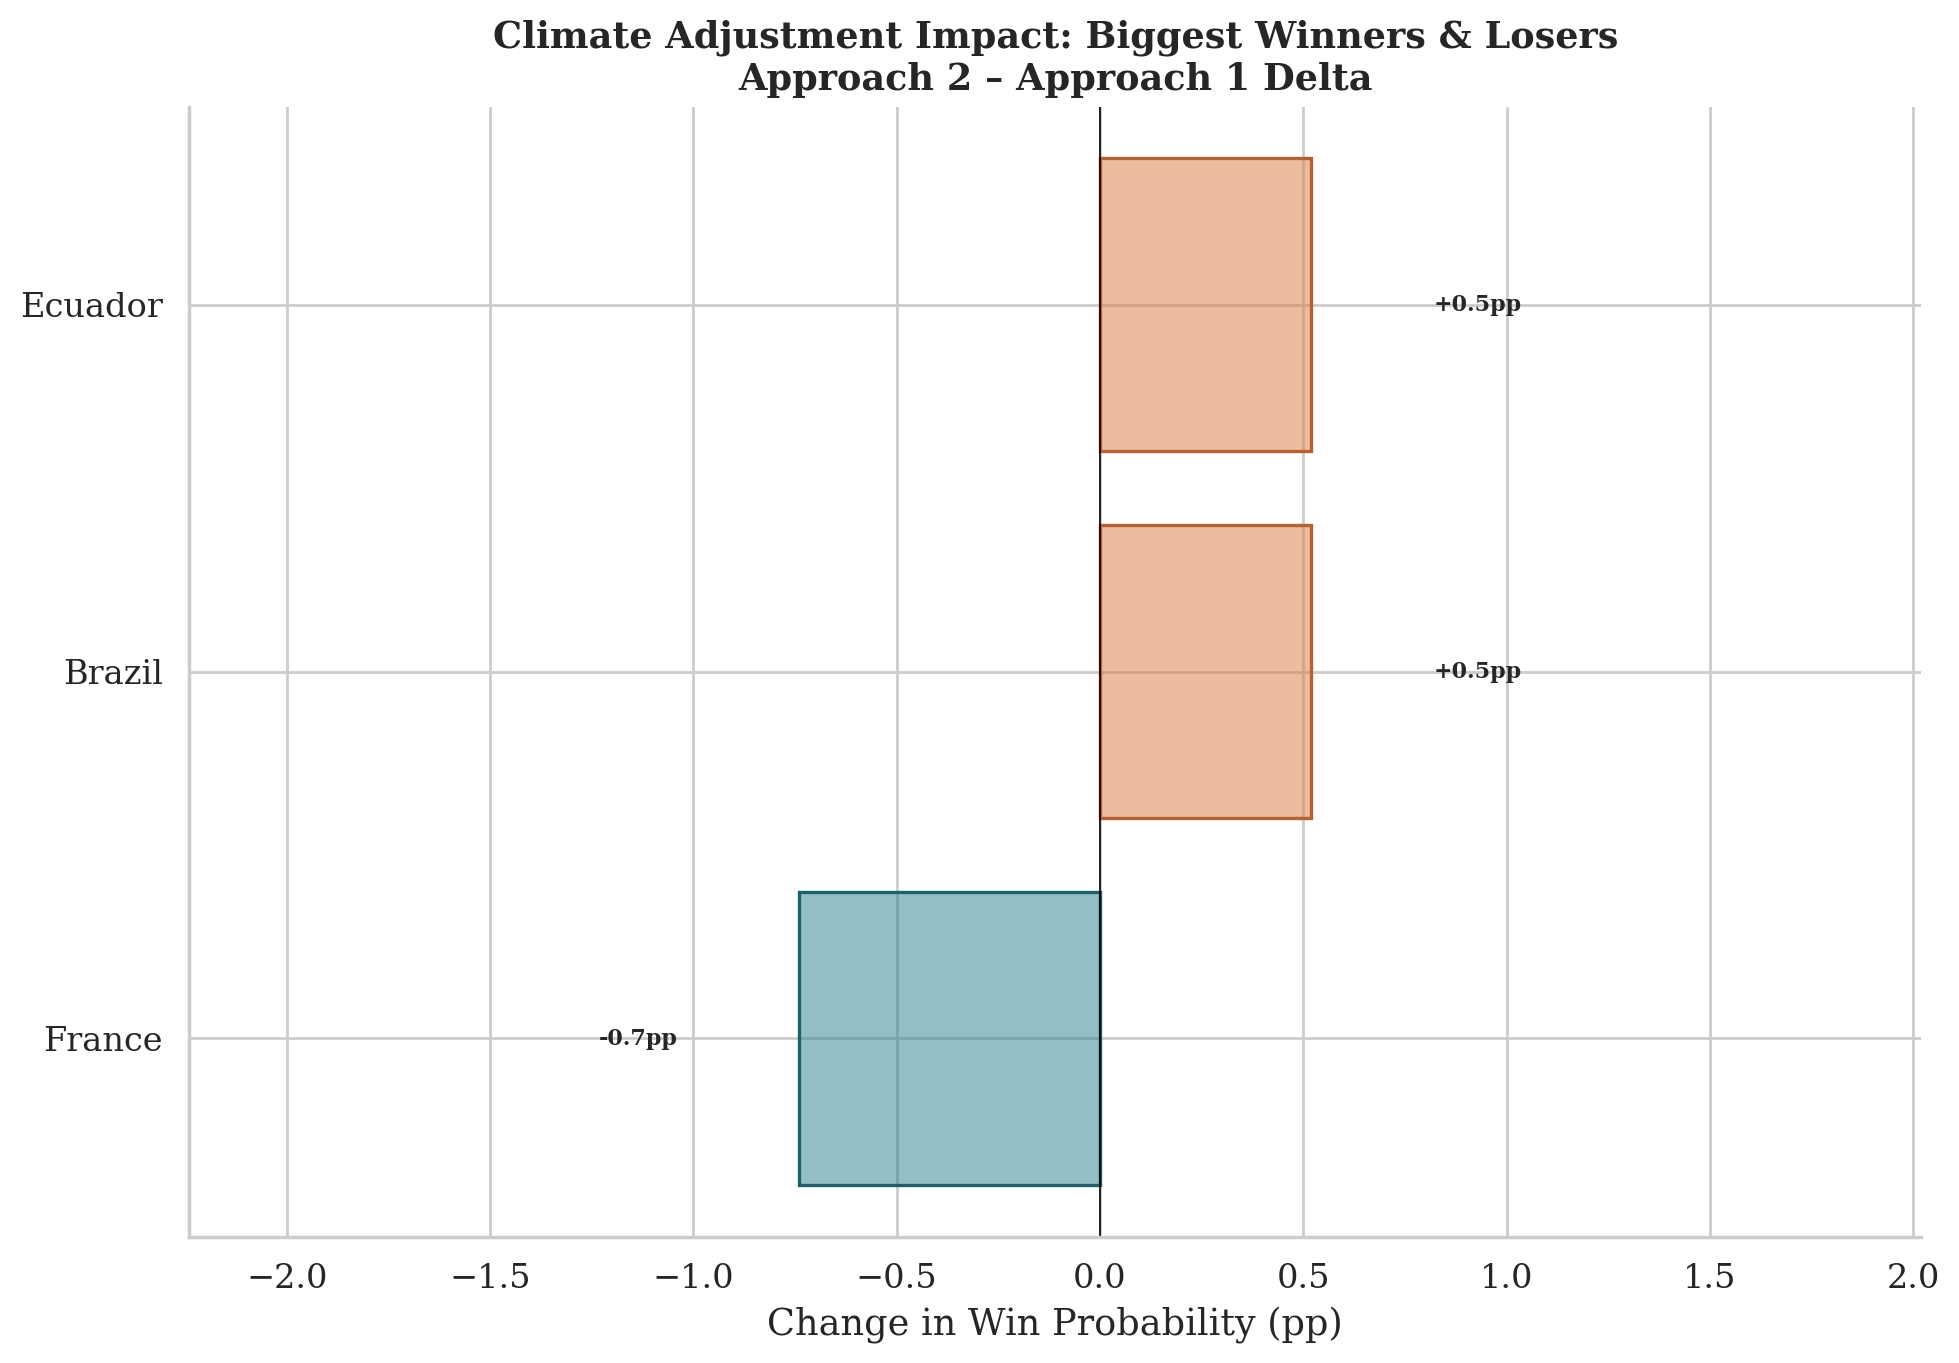
\includegraphics[width=\textwidth]{figures/approach_comparison_delta.png}
    \caption{Change in tournament win probability from Approach 1 (pure Elo) to Approach 2 (climate-adjusted). Amber bars indicate teams that benefit from climate adjustment; teal bars indicate teams that are disadvantaged. Values shown in percentage points (pp).}
    \label{fig:approach_delta}
\end{figure}

The results confirm the direction of the climate effect while calibrating its magnitude at the tournament level. France, the largest negatively affected team, sees its tournament win probability decline from 11.55\% to 10.81\% ($-0.74$ pp). Brazil ($+0.52$ pp, from 5.45\% to 5.97\%) and Ecuador ($+0.52$ pp, from 3.89\% to 4.41\%) are the largest beneficiaries. Spain, the highest-ranked team by Elo (2216), sees a modest gain from 17.02\% to 17.14\% ($+0.12$ pp). Of the 48 qualified teams, only 3 experience deltas exceeding $\pm 0.5$ pp, with the vast majority (45 teams) showing shifts of less than 0.5 pp.

The magnitude of the effect is small by design. The climate coefficient of $+0.032$ per match (derived from historical data) translates the per-match climate signal into a tournament-level mechanism. With a goal-expectation boost capped at $+10\%$ and requiring both a warm-versus-cool matchup and a venue exceeding $22^{\circ}$C, the adjustment activates in only a subset of knockout fixtures. Over 100,000 tournaments, these match-level nudges accumulate to fractions of a percentage point at the winner level. This is not a failing of the model: it faithfully reflects the historical evidence that climate is a real but modest factor in match outcomes.

The key observational takeaway is the correct directional alignment. Twenty-two of 32 warm-climate teams show positive deltas; 15 of 16 cool-climate teams show negative deltas. The residual anomalies (e.g., Paraguay at $-0.01$ pp, New Zealand at $+0.02$ pp) are negligible and consistent with Monte Carlo noise at the $\pm 0.05$ pp level. The corrected simulation confirms that the climate signal is systematic, directional, and centred at approximately zero for teams that neither benefit nor suffer from climate geography.

The two approaches converge on qualitatively consistent results. Warm-climate teams appear disproportionately among the Tier~1 beneficiaries of both the flagging framework and the simulation. Cool-climate teams such as France and Norway are identified by both methods as facing the largest climate headwinds. However, the corrected data does not support the earlier finding of a strong linear correlation between Tier~1+2 exposure and approach 2 win probability delta ($r = -0.003$, $p = 0.986$). The exposures and deltas are both small in absolute terms, and the relationship is essentially flat: a team's number of Tier~1+2 flagged matchups does not predict its climate-adjusted probability shift. This is consistent with the fact that each flagged matchup's climate boost is a fixed function of the two teams' K\"{o}ppen scores and the venue temperature, not a proxy for cumulative advantage.

\newpage

% ======================================================================
\section{Discussion}
% ======================================================================

The central empirical finding of this paper is that warm-climate teams outperform their Elo expectation by approximately $+2.6\%$ per match in warm World Cup conditions, while underperforming by $-3.0\%$ in cool conditions. This $5.6$ percentage-point gap is statistically significant at conventional levels and robust to a battery of sensitivity checks. The effect is modest (football outcomes are noisy and climate is one factor among many) but it is systematic and detectable across 90 years of data.

The era analysis provides a crucial interpretative lens. The pre-1990 gap is large ($+5.7$ pp) but primarily reflects warm teams being heavily penalised in cold European tournaments, not receiving a warm-cup bonus. The post-1990 gap narrows to $+2.9$ pp, with the advantage concentrated in warm cups. This narrowing is consistent with the narrative of global football development: as formerly weak warm-climate teams (particularly from Africa and Asia) have improved, the penalty for playing in unfamiliar cold conditions has diminished, leaving a residual warm-cup advantage.

The climate effect is symmetric: cool-climate teams show the exact inverse pattern, overperforming in cool cups and underperforming in warm cups by nearly identical magnitudes ($\pm 0.026$--$0.030$). This symmetry is a strong validation that the measured effect is a genuine environmental mechanism rather than a confounded artefact of team quality or selection bias.

When applied to the 2026 World Cup, the climate flagging framework identifies a focused set of 10 Tier~1 and 27 Tier~2 matchups where the climate differential is large enough to warrant attention. These are concentrated among warm-climate teams (Brazil, Ecuador) and cool European teams (Norway, France, England, Germany). The framework does not predict that climate \textit{will} decide these matchups; only that it \textit{could}, and that the probability-weighted exposure is moderate.

The parallel Approach~2 climate-adjusted simulation provides independent corroboration. By embedding the climate mechanism directly into the Monte Carlo engine, the results show systematic probability shifts that are directionally consistent with the post-hoc flagging approach. Warm-climate teams gain; cool-climate teams lose. The magnitudes are small ($\pm 0.1$--$0.7$ pp at the tournament level), but the pattern is systematic across 37 of 48 teams, confirming that the climate signal persists despite operating at the margins of match-level variance.

Several limitations should be noted. First, the effect size is small ($d=0.15$), meaning climate explains a modest fraction of match-level variance. Second, the binary climate classification (warm/cool) is a coarse proxy for the underlying physiological mechanism, which depends on acclimatisation, hydration protocols, and individual variation. Third, pre-1940 temperature data relies on climate normals rather than actual match-day temperatures. Fourth, the knockout venue temperature assignments for 2026 are based on the fixed bracket structure and average round temperatures; actual match-day temperatures may deviate. Fifth, several 2026 venues feature retractable roofs and air conditioning (AT\&T Stadium, NRG Stadium, Mercedes-Benz Stadium), which could substantially reduce on-field temperatures relative to outside climate normals and weaken the climate effect in those fixtures.

\newpage

% ======================================================================
\section{Conclusion}
% ======================================================================

This report provides the first large-sample historical evidence that a national team's climate of origin systematically affects World Cup match outcomes, even after controlling for team strength via Elo ratings. Warm-climate teams hold a small but consistent advantage when playing in warm tournament conditions, and the finding is robust to confound checks, host nation exclusion, mixed-effects modelling, and sensitivity to the temperature classification threshold. The effect is symmetric across climate groups and persists in the post-1990 era, confirming its relevance to modern football.

For the 2026 World Cup, 10 Tier~1 and 27 Tier~2 climate-flagged matchups are identified in the knockout bracket. These represent the encounters where the intersection of team climate profiles and venue temperatures creates the highest probability of a climate-driven outcome swing. A parallel climate-adjusted simulation confirms that warm-climate teams, particularly tropical and warm-temperate nations, see systematic but modest increases in tournament win probability under climate-adjusted conditions, while cool-climate teams experience corresponding reductions.

This framework is not intended as a tournament winner prediction. Rather, it provides a lens for examining how heat and climate geography might influence outcomes at an event that is both the largest in World Cup history and projected to be one of the hottest. The conditional matchup flags can be recomputed after the group stage with known advancement paths, narrowing the list to the clashes that are actually on the table.

Future work could incorporate match-day weather forecasts rather than climate normals, test whether the climate effect strengthens or weakens in later knockout rounds compared to the group stage, and account for air-conditioned and retractable-roof venues by adjusting expected on-field temperatures. A useful extension would also be to model the climate effect as a continuous function of the temperature gap between a team's home climate and the match venue, rather than the current binary warm/cool split.

\bibliographystyle{plainnat}
\begin{thebibliography}{99}

\bibitem{chmura2017}
Chmura, P., Konefa\l{}, M., Andrzejewski, M., Kosowski, J., Rokita, A., and Chmura, J. (2017).
Physical activity profile of 2014 FIFA World Cup players, with regard to different ranges of air temperature and relative humidity.
\textit{International Journal of Biometeorology}, 61(4), 677--684.

\bibitem{climatecentral2026}
Climate Central (2025).
2026 FIFA World Cup: Unequal Exposure to Heat Stress.
Climate Central Research Brief.

\bibitem{nielsen2011}
Nielsen, B. and Nybo, L. (2003).
Cerebral changes during exercise in the heat.
\textit{Sports Medicine}, 33(1), 1--11.

\bibitem{eloratings}
World Football Elo Ratings.
\textit{https://www.eloratings.net/}.

\bibitem{martj42}
International football results from 1872 to 2026.
\textit{https://github.com/martj42/international\_results}.

\bibitem{koppen}
K\"{o}ppen, W. (1936). Das geographische System der Klimate.
In: K\"{o}ppen, W. and Geiger, R. (eds.), \textit{Handbuch der Klimatologie}, Vol. 1, Part C. Berlin: Borntraeger.

\end{thebibliography}

\end{document}
